\documentclass[a4paper]{article}
\usepackage{float}
\usepackage[swedish]{babel}

\usepackage[fixlanguage]{babelbib}

\selectbiblanguage{swedish}
\usepackage[nottoc]{tocbibind}

\usepackage[T1]{fontenc}
\usepackage[utf8]{inputenc}
\usepackage{graphicx}
\usepackage{makecell}
\usepackage{hyperref}
\usepackage{pdfpages}
\usepackage[]{ragged2e}
\setlength\parindent{0pt} %changes indentation size to 0
\usepackage[toc,page]{appendix}

\begin{document}

\title{
  Säkerhetssystem med MD407 \\
  \large Utveckling av ett MD407-baserat säkerhetssystem med CAN-kommunikation}
\date{2020-11-01}

\author{ Philip Antonsson, Felix Bråberg, Linus Haraldsson,  Gabriel Käll,\\  Erik Nilsson, Sebastian Sjögren, Simon Widerberg \\Datatekniskt projekt}

\maketitle
\thispagestyle{empty}
\newpage
\thispagestyle{empty}
\newpage


%Ni skriver all text i projektplanen med ett projektinternt perspektiv.
%Detta betyder att ingenstans ska det framgå att projektet drivs inom
%ramen för en kurs i utbildningssyfte, utan att detta är ett renthttps://www.overleaf.com/project/5f5652a06c50130001db661f
%tekniskt utvecklingsprojekt.

%Eftersom de tre första avsnitten, Syfte, Mål och Bakgrund, återkommer
%(helt intakta, om de är välskrivna) i projektrapporten, tveka inte över

\tableofcontents
\pagenumbering{gobble}
\newpage
%Ordlista
\section*{Ordlista}
\label{sec:ordlista}
\begin{description}
    \item[Buss]{En elektrisk bana som används för dataöverförning mellan datorkomponenter \cite{collins:2014}.}
    \item[CAN(Controller Area Network)]{Ett asynkront protokoll för kommunikation mellan separata
     hårdvaruenheter\cite[s. 249]{lme:2016}.} %%\cite[pg 2]{corrigan:2016} bättre?
    \item[Discord]{En plattform för gruppsamtal över internet.}
    \item[GitHub]{Webbhotell för lagring av källkod.}
    \item[Gren]{En version av mjukvara som lagras på Github.}
    \item[IO]{Input-Output, representerar in- och utmatning av data.}
    \item[Ping]{En signal som begär ett svar från en enhet \cite{christensson:2016}.}
    \item[Struct]{En datastruktur, d.v.s. en bit av bestämt minne i datorn där data är grupperad och lagrad för lätt åtkomst.}
    \item[SysTick]SysTick är en timer baserad på hårdvarans klockcyklar som kan konfigureras för att regelbundet skapa avbrott.
    \item[USART]{Universal Synchronous/Asynchronous Reciever/Transmitter, en gränssnittsenhet som omvandlar data till bitströmmar. Används för att möjliggöra kommunikation mellan två hårdvaruenheter\cite{howe:2020}.}

\end{description}
\newpage
%Introduktion
\section{Introduktion}
\label{sec:intro}

\subsection{Syfte}
\label{sec:syfte}
\pagenumbering{arabic}
\setcounter{page}{1} % Set the page counter to 3

%Syftet beskriver koncist varför projektet ska genomföras och vad ett
%uppfyllande av de tekniska målen leder till.

%Vanligtvis är syftet så klart ledande för uppgiften man löser. Här är
%det lite tvärt om eftersom ni fått en uppgift och måste komma på ett
%syfte för den, men det ska nog gå bra.

%Ha gärna med lite fakta i syftesparagrafen. Istället för att bara skriva
%självklarheter som att det är bra med larm ifall det kommer tjuvar så
%kan man ha med några siffror på vad larmbranchen omsätter till exempel
%eller hur vanligt det är med inbrott eller något.
År 2018 var det cirka 82 000, eller 1,8 procent, av rikets hushåll som rapporterade fall av bostadsinbrott i Sverige. Detta antal var detsamma år 2016 och 2017 \cite{ntu:2019}. Enligt Statistiska centralbyrån har den vanligaste lägenhetstypen två rum och kök \cite{scb:2018}. Det är dock inte en majoritet som bor så, och bostadsstorlekar samt bostadstyper varierar. 
Därmed är det viktigt att säkra larm- och låssytem finns till för medborgares säkerhet, och att de är anpassade för deras bostäder. 
Projektets syfte är därför att ta fram ett larm- och låssystem baserat på mikrokontrollern MD407 som också är modulärt. 

%Avslutningsvis utväderades arbetet med hänsyn till funktinalitet, säkerhet och %vidarutveklingsmöjligheter. 
\subsection{Mål}
\label{sec:mål}
%I detta avsnitt beskrivs koncist samtliga övergripande tekniska mål med
%projektet, det vill säga, vad ska konstrueras. Mycket av det här
%framgår så klart i uppgiften.

%Se till att tydligt ange målsättningen vad gäller de extrauppgifter som
%finns tillgängliga i projektdirektiven. Ni kan dela upp eventuella
%extrauppgifter i två olika prioritetsgrader. Att ta på sig en massa
%extrauppgifter här som ni inte ens försöker genomföra är inte bra.
%Försök göra en realistisk bedömning av vad ni hinner med även om det är
%svårt.

%De mål som anges här kommer att styra projektets utveckling. När
%projektet närmar sig sitt slut och den slutliga projektrapporten lämnas
%in kommer beställaren (läraren i vårt fall) att kritiskt analysera hur
%väl projektet lyckats genom att jämföra planens mål med den tekniska
%konstruktion som redovisas i projektrapporten.

Projektets mål var att utveckla ett larm- och låssystem med hjälp av en centralenhet samt två periferienheter och en störenhet. De två periferienheterna var ett dörrlarm och ett rörelselarm. 
Övergripligt används periferienheterna för att interagera med de fysiska sensorerna och larmen. Centralenheten används för att hantera all information samt kommunikation. Störenheten användes för att stresstesta systemet. Enheterna skall kommunicera med varandra över en gemensam buss med hjälp av protokollet Controller Area Network (CAN).\ref{sec:ordlista} 
\newline\newline
Två utökningar av grundsystemet planerades. Den ena var att rörelselarmet inte skall larma till centralenheten förrän det befinner sig någon inom en viss variabel räckvidd från enheten. Alltså skall rörelselarmet endast larma lokalt tills räckvidden blir överskriden av någon. Den andra planerade utökningen var att ljudet som uppgör larmet skulle sticka ut och vara så tydligt som möjligt. Prioriteringen av utökningarna var i samma ordning som de introducerades.

\subsubsection{Kravspecifikation}
\label{sec:kravspec}
Följande kravspecifikation har utvecklats för att uppnå målet och täcka de nödvändiga funktionerna av ett säkerhetssystem:
\begin{enumerate}
    \item Enheterna ska kunna kommunicera genom CAN-bussen på ett konsekvent sätt.
    \label{itm:krav1}
    \item Centralenheten ska lagra aktuell information om alla enheter.
    \label{itm:krav2}
    \item Centralenheten ska presentera den viktigaste informationen för 
    användaren genom USART, Universal Synchronous/Asynchronous Reciever/Transmitter.
    \label{itm:krav3}
    \item Periferienheterna ska vara konfigurerbara genom USART.
    \label{itm:krav4}
    \item Det globala larmet ska utlösas ifall centralenheten förlorar kontakten med en periferienhet.
    \label{itm:krav5}
    \item Periferienheterna ska tillämpa ett lokalt larm om sensorer blir triggade, och larma globalt om det behövs.
    \label{itm:krav6}
    \item Om larmet har gått kan det avaktiveras från centralenheten genom att en kod matas in på en knappsats.
    \label{itm:krav7}
    \item Användaren ska kunna koppla upp systemet med de periferienheter som behövs, och inte vara låst till en speciell konfiguration.
    \label{itm:krav8}
\end{enumerate}
Punkt ett togs fram för att ett system behöver förutsägbar kommunikation för att vara pålitligt. Annars kan en mängd problem uppstå, som att sidoeffekter förekommer vid konfiguration, e.t.c. Punkt två ansågs också vara väsentlig; att bedöma när ett larm ska utlösas kräver aktuell information om systemet. För att användaren ska kunna ta del av denna aktuella information måste den presenteras genom USART på ett förståeligt sätt. Informationen presenteras för användaren så den kan konfigurera perifirienheterna genom USART. Därför behövs punkt tre och fyra som krav.
De tre punkterna innan punkt åtta är relaterade till systemets primära funktion - att larma på och av vid rätt tillfälle. Därför är krav fem, sex och sju nödvändiga för ett fungerande system. 
Punkt åtta är obligatorisk för systemets modularitet, och krävs därför i detta larmsystem.

\subsection{Arbetsmetod}
\label{sec:arbetsmetod}
Arbetet delades i början av projektet upp i åtta delar, vilka beskrivs i sektion \ref{sec:Design}. Varje gruppmedlem blev tilldelad en primär deluppgift samt en eller flera närliggande uppgifter att assistera med. 
\newline \newline
Projektets mjukvara kodades i C med hjälp av textredigeraren Codelite. Tre enheter med olik funktionalitet skulle utvecklas, och det bestämdes att en uppsättning kod per enhet var optimalt. Detta gjorde mjukvaruutvecklingen mer effektiv eftersom koden för de tre enheterna kunde skrivas parallellt, och tester kunde utföras individuellt innan systemets sammankoppling. Testerna på enheternas mjukvara utfördes i hierarkisk ordning. De minsta delarna av programmen testades först, eftersom dessa delar inte förlitar sig på någon annan kod. Efter det testades större och större block av kod, och till slut hela enheten. Testerna på enhetsnivå dokumenterades och diskuteras i avsnitt \ref{sec:resultat}.
\newline \newline
För att abstrahera bort svårskriven lågnivåkod användes ''STM32F4xx Standard Peripherals Library''. Det är ett programvarubibliotek för processorn i MD407 som underlättar användningen av diverse hårdvara som enheten stödjer. En del hårdvara tillhörande till dörrenheten och larmenheten behövdes dock utvecklas på egen hand. Den utvecklades med hjälp av en kopplingsplatta, el-komponenter, och egenskrivna funktioner. 
\\ \\
Arbetet på de enskilda delenheterna skedde på separata grenar i github. Om en gren skulle slås ihop med master grenen krävdes att följande kriterier uppfylldes.
\begin{enumerate}
    \item Koden var godkänd av en annan gruppmedlem.
    \item Om en skriven funktion inte var trivial krävdes en testfunktion för att bevisa dess funktionalitet.
    \item Koden jämfördes mot och rättades efter kodkonventionsdokumentet. 
    \item Funktionalitetstester utfördes och testdokumenten bifogades.
\end{enumerate}


\newpage
%Teknisk bakgrund


\section{Teknisk bakgrund}
Detta kapitel ger en teoretisk översikt över de grundläggande komponenterna i larmsystem, och hur de fungerar. I samband med detta förklaras en del av hårdvaran som används i projektet ingående. Efter det beskrivs teorin bakom kommunikationstandarden CAN. 
\label{sec:tekniskbakgrund}
\subsection{Larmsystem}
Larmsystem kan variera när det gäller utrustning och komplexitet, men det finns gemensamma komponenter som utgör en bas för systemen. Denna bas består ofta av \textit{sensorer}, \textit{centralutrustning} och \textit{larmdon} \cite[s. 15]{lundh:2008}.  
%REFERERA TILL DENNA BOK IST
%VAD GÖR MAN OM BOKEN HAR ETT ANNAT ORD FÖR CENTRALENHET
%https://www.bokus.com/bok/9789188816108/larm-overvaknings-och-sakerhetssystem-faktabok/
Sensorerna är larmsystemets ''sinnen''. Deras uppgift är att upptäcka ändringar i tillstånd. Tillstånden kan vara tryck, ljud, ljus, slutande eller brytande kontakt, \cite[s. 15]{lundh:2008}. 
Denna ändring i tillstånd signaleras till centralutrustningen genom systemets kommunikationsstandard. Ett gemensamt kommunikationsprotokoll används för det valda mediet. \newline \newline 
Om sensorerna är larmsystemets ''sinnen'' är centralutrustningen larmsystemets ''hjärna''. Centralenheten tar emot information från sensorerna, och dess uppgift är att tolka vad denna information betyder \cite[s. 18]{lundh:2008}. När centralenheten har tolkat informationen bestämmer den vad som ska göras härnäst. Om någon av sensorerna har gett ett oroväckande utslag kanske centralenheten skickar en signal till ett larmdon. 

\subsection{Projektets kommunikationstandard, CAN}
\label{sec:can}
CAN, Controller Area Network, är en databuss som utvecklades för fordonsindustrin. Denna buss tillåter kommunikation mellan flera enheter, där alla enheter delar samma kommunikationsmedium. Protokollet har också förmågan att självdiagnostisera och reparera fel i meddelanden. \begin{flushright}
\cite[s. 2]{corrigan:2016}
\end{flushright} 
För att förhindra och alternativt optimera kollisioner använder sig CAN av protokollet CSMA/CD+AMP. Detta protokoll gör så att noder ''lyssnar innan de pratar'', de väntar en specificerad tid innan de börja sända information. Om en kollision skulle uppstå används meddelandenas prioritet för att lösa den – meddelandet med högre prioritet fortsätter att sända. När ett larmsystem utvecklas kan detta användas till systemets fördel; utvecklare kan definera att larmmeddelanden alltid har högsta prioritet. \begin{flushright}
\cite[s. 3]{corrigan:2016}
\end{flushright} 

CAN-meddelanden är förpackade i så kallade CAN-ramar och har en standardiserad struktur. Den CAN-ram som anses vara av standardstruktur visualiseras i figur \ref{fig:can_frame}. Diverse fält i ramen beskrivs nedan:
\begin{description}
    \item[ID-fältet] {Innehåller meddelandets ID.}
    \item[Reserverat] {Innehåller information angående vad för typ av ram det är samt vilket typ av ID ramen använder sig av.}
    \item[Längd] {Längden på databufferten i bytes.}
    \item[Data Buffert] {Bufferten där all data ligger. Längd-fältet beskriver databuffertens storlek.}
    \item[CRC-fältet] {\emph{Cyclic Redundancy Check} är en felkontrollskod. Den används för att undersöka om ett meddelande har kommit fram oskadat.}
    \item[ACK] {\emph{Acknowledge} skickas av mottagande noder för att tala om för avsändarnoden att meddelandet kom fram. }
\end{description}
\begin{figure}[h]
    \centering
    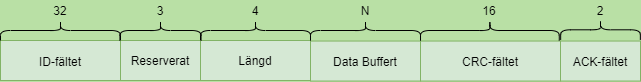
\includegraphics[scale=0.52]{dokumentation/projektrapport/IMAGES/can_frame.png}
    \caption{En CAN-ram av standardstruktur. Talen beskriver antalet bytes. N innebär att databuffertens längd kan variera. Den bestäms av värdet i längd-fältet.}
    \label{fig:can_frame}
\end{figure}


\subsection{Projektets sensortyper}
\label{sec:sensortyper}
%I detta projekt används tre typer av sensorer: magnetkontakter, %vibrationssensorer och avståndssensorer. Magnetkontakten som används %består av två delar: en magnet och en mekanisk kontakt. Om kontakten %är kopplad till en elektrisk krets hålls kretsen sluten, så länge %magneten är nära den (Nästan så de vidrör varandra). Denna sensor %fungerar utan någon strömtillförsel. [a.a] I projektet tillämpas %denna funktion i dörrenheten.
I detta projekt används tre typer av sensorer: en magnetkontakt, en vibrationssensor och en avståndssensor. Magnetkontakten som används består av två delar: en magnet och en mekanisk kontakt. Kontakten påverkas av magnetens fält, och om denna är kopplad till en elektrisk krets, kan denna krets slutas eller brytas \cite[s. 15]{lundh:2008}. Så länge magneten är nära kontakten hålls kretsen sluten, och sensorn behöver ingen strömförsörjning för att detta ska fungera. Det här används för att kontrollera om en dörr är stängd. 
\newline \newline
Till skillnad från magnetkontakten behöver resten av sensorerna strömförsörjning.
Vibrationssensorn som används kallas \textit{SW-18010P}. Sensorn har en liten fjäder innanför sitt metallskal, och när denna fjäder vidrör skalet sluts kretsen. Den reagerar därför på rörelse och vibration från alla möjliga riktningar. I projektet används det för att detektera inbrott, t.ex. att en ruta krossas.
Avståndssensorn \textit{HC-SR04} använder ultraljud för att rapportera hur nära något är i dess synfält. Sensorn avger ultraljudsvågor, och mäter hur lång tid det tar dem att komma tillbaka. Tiden och frekvensen av vågorna används för att uppskatta hur långt de färdades. Den kan mäta avstånd från 2 till 400 centimeter med upp till tre millimeter exakthet, och används för att detektera om någon eller något närmar sig. 
\begin{flushright} 
\cite{elecfreaks} , \cite{bailing:2011}
\end{flushright}



\newpage
\subsection{MD407 - En översikt}
\label{sec:md407}
Mikrokontrollern MD407 har många anslutningsportar på sitt kretskort. Här beskrivs de portarna som är relevanta för projektet, och var de befinner sig (se figur \ref{fig:md407}).

\begin{figure}[h]
    \begin{center} 
    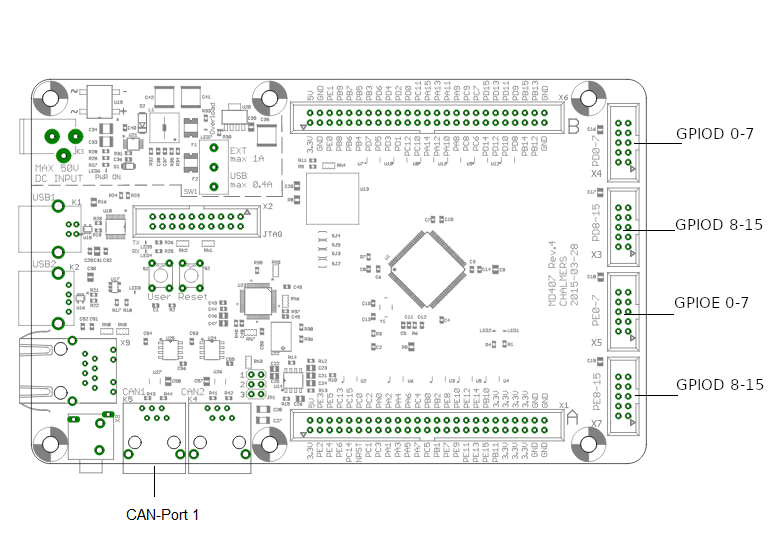
\includegraphics[scale=0.55]{dokumentation/projektrapport/IMAGES/md407.png}
    \caption{Portar på MD407 som är relevanta för projektet. De gröna cirklarna inuti GPIO-portarna representerar en anslutningspunkt, där en kabel kan anslutas. En anslutningspunkt kan beskrivas som en ''pin'' \cite{md407}.}
    \label{fig:md407}
    \end{center} 
    ''CAN-port 1'' används för att koppla samtliga enheter till CAN-bussen. GPIO-portarnas nummer refererar till vilka ''pinnar'' portarna har: GPIOD 0-7 har pinnar 0-7.
\end{figure}
\newpage
\newpage
%Design
\section{Design}
\label{sec:Design}

För att säkerhetssystemet ska fungera korrekt måste det klara av en mängd olika uppgifter. Bland annat: kontrollera om en dörr är öppen; avljuda larm; läsa och tolka värden från sensorer, och ta emot inmatning av användare. Systemet delas upp i moduler för att effektivt utföra de nödvändiga funktionerna. Detta underlättar även utvecklingen av projektet. En grafisk översikt av systemet visas nedan i figur \ref{fig:systemoversikt}. Rektanglarna är moduler och pilarna är de funktioner som anropas mellan dem.

\begin{figure}[H]
    \centering
    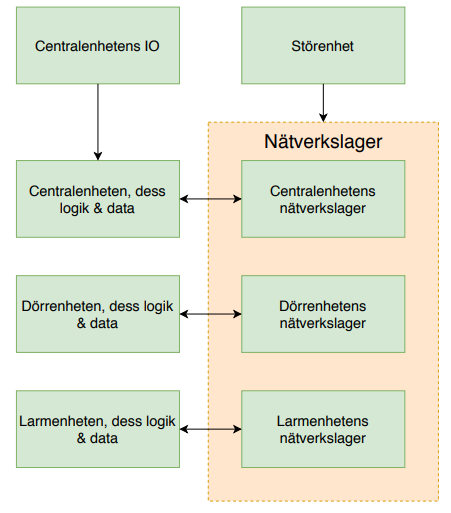
\includegraphics[scale=0.75]{dokumentation/projektplan/systemoversikt.png}
    \caption{Grafisk representation av systemet}
    \label{fig:systemoversikt}
\end{figure}


\subsection{Nätverklagret}
\label{sec:nätverklagretDE}
Ett CAN-protokoll designades för projektet. Den ram som designades syns
i figur \ref{fig:can_frame_own}. ID-fältet innehåller identifieringsinformation för meddelandet. RTR(Remote Transmission Request) innehåller information angående typen av ram. IDE(Identifier Extension) säger vilken typ av identifiering som ramen har. Längd ger längden på databufferten och databuffert
innehåller datan i fråga. Databufferten kan som längst vara åtta bytes lång. Utöver protokollet planerades också ett bibliotek för användandet av CAN. Ett sådant bibliotek hjälper uppfyllandet av krav ett under \ref{sec:kravspec}.

\begin{figure}[h]
    \centering
    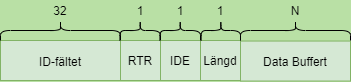
\includegraphics[scale=0.7]{dokumentation/projektrapport/IMAGES/can_frame_own.png}
    \caption{Den designade CAN-ramen}
    \label{fig:can_frame_own}
\end{figure}
\newpage

ID-fältet innehåller i sin tur data om meddelandet. Fältet visualiseras i figur \ref{fig:id_fält}. Samtliga sektioner i fältet beskrivs nedan:
\begin{description}
    \item[DIR] är meddelandets riktning. Är biten satt till noll är meddelandet ämnat till centralenheten. Är biten ett så är meddelandet från centralenheten.
    \item[Message ID] är meddelandets ID. Den säger vad det är för slags meddelande som skickats.
    \item[Node ID] har olika betydelser beroende på vad DIR-biten är satt till. Är DIR-biten satt till noll säger detta fält vilken enhet meddelandet är ämnat för. Men om DIR-biten är satt till ett beskriver fältet vilken nod meddelandet kom ifrån.
\end{description}
\begin{figure}[h]
    \centering
    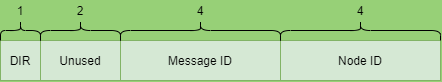
\includegraphics[scale=0.6]{dokumentation/projektrapport/IMAGES/protocol_new.png}
    \caption{CAN-ramens ID-fält, talen beskriver antalet bytes.}
    \label{fig:id_fält}
\end{figure}

Det fanns olika sorter av meddelanden som designades. Dessa syns tabell \ref{tab:msg_types} nedan. Genom att ha olika meddelandetyper blir det lättare att skriva hanteringsfunktioner för CAN-meddelanden då programmet utför rutiner baserat på typerna. Prioriteringen av diverse meddelandetyper är densamma som ordningen i tabellen, där högsta prioriteten är längst upp i tabellen.

\begin{table}[h]
    \caption{Alla typer av meddelanden. Högst prioritering längst upp i tabellen.}
    \begin{center}
     \begin{tabular}{ |c p{8cm}| }  
     \hline
     Typ & Betydelse  \\ [0.5ex] 
     \hline\hline
     Alarm & Säger åt larmenheten att den ska slå larm. \\ 
     \hline
     Ping & Ett vanligt pingmeddelande. När en periferienhet får ett pingmeddelande lägger enheten upp ett eget pingmeddelande på bussen som svar. \\
     \hline
     Konfigurering & Innehåller nya konfigurationer till en enhet. \\
     \hline
    \end{tabular}
    \end{center}
    \label{tab:msg_types}
\end{table}


\subsection{Centralenheten}
\label{sec:centralenhetenDE}
Om man sammanfattar centralenhetens uppgift ska den fungera som administratör för alla enheter. I \ref{sec:kravspec} nämns det att den ska lagra aktuell information om dessa och konfigurera om dem, men också att den ska larma om någon enhet blir frånkopplad. För att uppfylla dessa krav designades centralenhetens logik efter flödesschemat som visas i figur \ref{fig:centralflöd}. Datahanteringen utvecklades enligt kravspecifikation två, och logiken gällande enheterna enligt kravspecifikation fem.
\newline \newline
\begin{figure}[h]
    \centering
    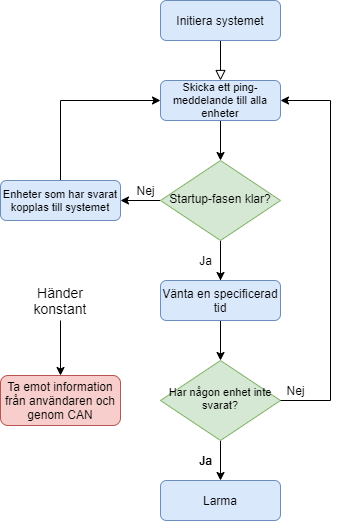
\includegraphics[scale=0.6]{dokumentation/projektrapport/IMAGES/centralenhet_flowchart.png}
    \caption{Flödesschema för centralenhetens logik}
    \label{fig:centralflöd}
\end{figure}
\newline \newline
I schemat beskrivs det att data konstant tas emot från användaren och CAN. Denna information handlar mest om de kopplade enheterna, och behöver lagras, både för användaren och systemet i helhet. Därför använder sig centralenheten av en lista, där varje plats i den innehåller information om en kopplad modul. Informationen inuti listan är en ''struct'', en datarepresentation av modulen. Dessa ''structs'' underlättar när specifik information ska hämtas gällande modulerna, och detta görs väldigt ofta i systemet.
\newline \newline
Schemat beskriver också centralenhetens logik; hur centralenheten kopplar enheter till systemet och detekterar om någon av dem blir frånkopplade. När uppstarts-fasen är klar är alla enheter anslutna till systemet, förutsatt att de svarade på ping-meddelandena som skickades. Centralenheten börjar då regelbundet skicka ut ping-meddelanden, väntar en specificerad tid, och undersöker om någon enhet inte har svarat i tid. Då larmar centralenheten globalt. Det här säkerhetsställer att inga delar av systemet kan kopplas bort utan att ett larm går.
\newline \newline
Uppstarts-fasen är designad med avseende på modularitetskravet (krav åtta). Systemet är inte ''låst'' till en speciell uppsättning enheter; alla som svarar på centralenhetens ping-meddelanden blir anslutna. Användningen av listan med ''structs'' möjliggör denna process. Teoretiskt sett kan en godtycklig mängd enheter av varierande typ kopplas till systemet. Detta underlättar också för användaren - systemets delar är anslutna så fort uppstart-fasen är färdig, utan någon konfiguration.

\subsection{Centralenhetens IO}
\label{sec:centralenhetIODE}
% används för att ta emot en kod användaren har slagit in för att stänga av larmet vilket sedan vidarebefordras till centralenheten som verifierar koden. USART används för att ge kommandon och konfigurera moduler. USART används även som en utport där programmet kan skriva ut statusmeddelande för att simplifiera debugging-processen.
%\newline\newline
Centralenheten IO består av en knappsats och USART. IO funktionerna för dessa utvecklades enligt kravspecifikation \ref{itm:krav3}, \ref{itm:krav4} och \ref{itm:krav7} (se \ref{sec:kravspec}). Därmed är knappsatsen designad för ta emot en sifferkod samt att lagra den för centralenhetens användning. USART utformades dels för att skicka utmatningar från centralenheten som presenteras för användaren. USART designades även för att ta emot inmatningar från användaren vilket tillåter konfigurationer och status meddelanden. Konfigurationerna sker via olika kommandon som användaren kan skriva in i USART. \\

Både knappsatsen och USART utvecklades för att inte avbryta programmet, vilket tillåter ett kontinuerligt program där alla funktioner kan köras vid alla tidpunkter. Detta krävs för en korrekt fungerande centralenhet då ping meddelanden måste mottas och hanteras konstant. (\ref{sec:centralenhetenDE}, figur \ref{fig:centralflöd}).

% Design IO = motivera och förklara grundläggande USART och knappsats funktioner, dvs bufferten, referera till centralenheten + krav för varför det behövs.  Systemet skall kunna hantera inmatningar ifrån USART och keypad samtidigt som den kör.

% Teknisk bakgrund IO = implementation av USART, säg buffertsystem, anledningen till buffersystemet finns redan.  

\subsection{Dörrenheten}
\label{sec:dörrenhetenDE} % cant write des:door, maybe try sec:doorDE
Säkerhetssystemet designades för att kunna hantera flera dörrar. Ett alternativ hade varit att ha en dörr per MD407-kort. Dock, eftersom att ett MD407-kort har förmågan att hantera ett flertal dörrsensorer utnyttjas det. Då blir det enklare samt effektivare att koppla upp ett större antal dörrar. Antalet uppkopplade dörrar bestäms i centralenheten. Varje dörr förses med ett unikt ID för att kunna skilja dem åt samt konfigurera dem separat. Konfigurationen sker genom att det skickas och mottages meddelanden över CAN med hjälp av CAN-protokollet i enlighet med krav ett och fyra (\ref{sec:kravspec}).
\newline\newline
En dörrs larmfunktion kan aktiveras och avaktiveras. En avaktiverad dörr signaleras med en grön diod. 
Enligt kravspecifikationen har dörrenheten både lokalt och globalt larm. 
Det lokala larmet, en röd diod, går efter dörren varit öppen längre än en given tid. 
Det används för att inte larma globalt i onödan. 
Exempelvis i fallet att dörren öppnas av misstag och sedan omedelbart stängs igen. 
Meddelande om globalt larm skickas till centralenheten då dörren varit öppen längre än en ytterligare angiven tidsgräns. 
Centralenheten avgör sedan hurvida larmenheten ska tjuta. Hur lång tid innan globalt samt lokalt larm ges kan konfigureras via CAN.

\subsection{Larmenheten}
\label{sec:LarmenhetenDE}
Larmenhetens huvudsakliga uppgift är att utlösa ett ljudbaserat larm om rätt krav möts. Dessa krav är antingen att centralenheten skickar ett meddelande över CAN om att utlösa larmet eller att larmenhetens sensorer har mätt ett visst värde. Sensorerna består utav en vibrationssensor  och en avståndssensor som skickar mätdata till larmenheten.
\newline\newline
Kommunikationen från Centralenheten via CAN-bussen har högsta prioritet eftersom även centralenheten snabbt måste kunna utlösa larmet vid behov. Det har ordnats genom att mottagna meddelanden skapar avbrott i systemet. Avbrottshanteraren för vidare meddelandet till en hanteringsfunktion beroende på vilken typ av meddelande det är. De meddelandetyper som hanteras är konfigureringsmeddelanden enligt krav fyra (\ref{sec:kravspec}), meddelanden för att växla av/på larmet och pingmeddelanden. 
\newline\newline
Enligt krav sex (\ref{sec:kravspec}) har larmenheten en utbyggnad i form av ett lokalt larm. Detta lokala larm består av en lampa som tänds när någon eller något närmar sig avståndssensorn. Syftet för utbyggnaden är att det ska avråda folk från handlingar som skulle leda till ett globalt larm. \\

\subsection{Störenheten}
\label{sec:störenhetenDE}
Störenheten utvecklades för att simulera en defekt periferienhet genom att skicka stora mängder data på CAN-nätverket. Enheten kan skicka faktiska meddelanden eller slumpad data. Förmågan att skicka båda typer utvecklades för att ha möjlighet att testa en bredare mängd problem som skulle kunna uppstå.

%referera till detta?%
\iffalse
\begin{enumerate}
    \item Enheterna ska kunna kommunicera genom CAN-bussen på ett konsekvent sätt.
    \label{itm:krav1}
    
    \item Centralenheten ska lagra aktuell information om alla enheter.
    \label{itm:krav2}
    
    \item Centralenheten ska presentera den viktigaste informationen för användaren genom USART.
    \label{itm:krav3}
    
    \item Periferienheterna ska vara konfigurerbara genom USART.
    \label{itm:krav4}
    
    \item Centralenheten ska larma ifall någon periferienhet går sönder eller blir frånkopplad.
    \label{itm:krav5}
    
    \item Periferienheterna ska tillämpa ett lokalt larm om sensorer blir triggade, och larma globalt om det behövs.
    \label{itm:krav6}
    
    \item Om larmet har gått kan det avaktiveras från centralenheten genom att en kod matas in på en knappsats.
    \label{itm:krav7}
    
\end{enumerate}
\fi
\newpage
%Teknisk beskrivning
    \section{Teknisk beskrivning}
\label{tekbeskrivning}

%Genom att det fyller i de kompetensluckor som en typisk läsare har,
%underlättar bakgrundstexten läsandet av konstruktionsavsnitten. Precis
%som avsnitten Syfte och Mål ovan kan detta avsnitt med fördel
%återanvändas i den slutgiltiga projektrapporten. När det gäller
%projektplanen för DAT290 beskrivs här bakgrunden till projektet vad
%gäller tillämpningen, dess sammanhang och de tekniska förutsättningar
%som råder. För att beskriva tillämpningen och dess sammanhang behöver ni
%förklara hur system av den typen som ska konstrueras här fungerar i
%största allmänhet.

%Men vem är den typiska läsaren? Man får förutsätta att läsaren har en
%viss teknisk kompetens, annars blir bakgrundsavsnittet alltför långt.
%Denna gränsdragning (“hur elementärt ska jag förklara vad jag gör?”)
%upplevs som ett svårt moment när man som student börjar skriva tekniska
%rapporter. En användbar regel är att vi utgår från att läsaren har, i
%stort sett, samma utbildning som rapportskribenten, men saknar
%specialistkunskap om projektets tillämpning.

Denna sektion beskriver hur projektets delsystem implementerades utefter systemets design och krav.
Systemet är uppdelat i moduler enligt figur \ref{fig:systemoversikt}. Nedanstående rubriker går in i mer detalj om respektive modul.



%\subsubsection{Nätverkslagret}
%\label{sec:nätverkslagret}
%Nätverkslaget tar hand om kommunikationen mellan enheterna, vilket  sker %över en CAN-buss (Controller Area Network). Alla enheter som använder sig %av CAN-bussen skickar och tar emot meddelanden med hjälp av protokoll som %utvecklades under projektets gång. Kommunikationen sker igenom %centralenheten.
%\newline\newline
%För att åstadkomma flexibilitet och modularitet skrevs ett CAN-bibliotek. %Biblioteket innehåller funktioner som skickar samt hanterar mottagande av %CAN-meddelanden. Biblioteket kan användas på alla periferienheter men %funktioner för att hantera enhetsspecifika meddelanden måste manuellt %imlementeras. 
%\newline\newline
%Ett CAN-meddelande består av 4 bytes av data samt en 8 bytes buffert för %resterande data. Det första byte-segmentet berättar huruvida meddelandet %kommer från eller till centralenheten, den andra berättar meddelandets %typ, den tredje berättar ID:et på noden som skickat meddelandet och den %fjärde talar om längden på meddelandets databuffert(i bytes).
%\newline\newline
\subsection{Nätverkslagret}
\label{sec:nätverkslagret}
För att standardisera hur meddelanden skickas och tas emot skrevs ett CAN-bibliotek. Biblioteket innehåller funktioner som skickar samt hanterar mottagande av CAN-meddelanden. Biblioteket kan användas på alla periferienheter men funktioner för att hantera enhetsspecifika meddelanden måste manuellt implementeras.
\newline\newline


\begin{figure}[h]
    \centering
    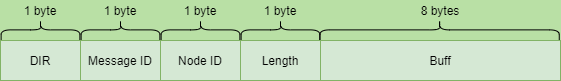
\includegraphics[scale=0.6]{dokumentation/projektrapport/IMAGES/can_msg_struct.png}
    \caption{Structen som representerar ett CAN-meddelande.}
    \label{fig:can_msg_struct}
\end{figure}

I koden skapades också en struct som representerade ett CAN-meddelande. Denna struct bestod av fyra bytes av riktnings- och destinationsdata samt längd på databufferten. Efter dessa finns det en buffert på åtta bytes för resterande data. Det första byte-segmentet beskriver huruvida meddelandet kommer från eller till centralenheten, det andra beskriver meddelandets typ, och det tredje representerar CAN-ramens ID och det fjärde talar om längden på meddelandets databuffert(i bytes). En visualisering av structen finns i figur \ref{fig:can_msg_struct}.
\newline\newline
Meddelandetyperna, som nämns i tabell \ref{tab:msg_types}, har definierats som konstanta heltalsvärden i koden. Prioriteringen av meddelandetyperna räknas ut genom en summering av ID för noden i meddelandet och ID för meddelandetypen. 



\subsection{Centralenhetens logik och datahantering}
\label{sec:centrallogik}
%%Fixa finare intro
När systemet startas aktiverar centralenheten en ''uppstarts-fas''. Den inleds med att centralenheten skickar ut ett ping-meddelande till alla enheter. När centralenheten märker att den har fått ett svar extraherar den informationen från meddelandet, skapar en datarepresentation av modulen, och lägger in den i en lista. Informationen som läggs in är bland annat modulens unika ''id'' och modulens typ, etc. Om en modul inte rapporterar inom tidsramen för uppstarts-fasen läggs den inte in i listan. Då ignoreras följande meddelanden från denna modul.
\newline \newline
Efter uppstarsfasen är klar skickar centralenheten ping-meddelanden till alla enheter varje sekund. Om en av enheterna inte hinner svara innan nästa meddelande skickas, sänder centralenheten en larmsignal till alla larmenheter. En larmsignal skickas också om centralenheten märker att dörrenheten larmar, och dörren i fråga är aktiverad.
\newline \newline
För att lagra information gällande modulerna använder sig centralenheten av en speciellt utformad datatyp. Datatypen och dess fält beskrivs i figur \ref{fig:module}. 
\begin{figure}[h]
    \centering
    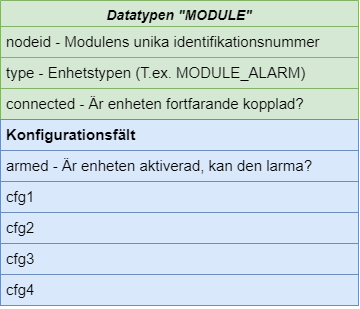
\includegraphics[scale=0.5]{dokumentation/projektrapport/IMAGES/diag_module.png}
    \caption{Datatypen ''MODULE'', gröna fält är konfigurationsfält.}
    \label{fig:module}
\end{figure}
\label{sec:centralenhetDL}
\begin{figure}[h]
    \centering
    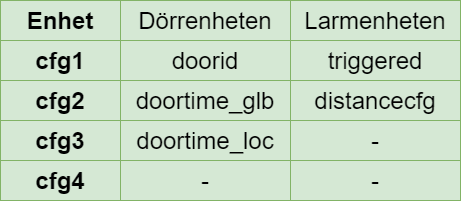
\includegraphics[scale=0.5]{dokumentation/projektrapport/IMAGES/cfg_fields.png}
    \caption{Modulernas konfigurationsfält, '-' betyder att fältets värde är odefinerat.}
    \label{fig:cfg}
\end{figure}

Konfigurationsfälten beskriver modulens nuvarande inställningar. Det första fältet beskriver om enheten är larmad eller inte, och resten beror på vilken modultyp enheten är. I figur \ref{fig:cfg} beskrivs det vad ''cfg1'' till ''cfg4'' representerar för detta projektets moduler. \\ \\
Dörrenhetens ''doorid'' anger hur många dörrar som dörrenheten är konfigurerad för. De följande fälten, localtime och globaltime är hur länge en dörr kan vara öppen innan dörrenheten slår lokalt respektive globalt larm. 
När det gäller larmenheten är ''cfg1'' ''triggered'', och beskriver om larmet är triggat. Det andra fältet representerar vilket avstånd som avståndsmätaren ska larma vid. Värdet i detta fält kan vara från 1-255, mätt i centimeter. %maxavståndet för sensorn (se \ref{sec:sensortyper}). Resten av fälten (''cfg3'', ''cfg4'') lämnas %tomma för båda enheterna. 

\subsection{Centralenhetens IO}
\label{sec:centralenhetIO}

%Centralenhetens knappsats används för att ta emot en kod användaren har slagit in. Koden vidarebefordras sedan till centralenheten som verifierar koden och stänger av. USART används för att ge kommandon och konfigurera moduler. USART används även som en utport där programmet kan skriva ut statusmeddelande för att simplifiera debugging-processen.
%\newline\newline
%Eftersom centralenheten tar emot information från flera olika källor är det viktigt att funktionerna som hanterar IO från knappsatsen och USART kan löpa kontinuerligt.  

%ett att alla inmatningar kan registreras och skickas vidare på kort tid används ett buffertsystem för båda enheterna

%Centralenheten kräver ett kontinuerligt system, där ingen funktion avbryter programmet (\ref{sec:centralenhetIODE})..

Centralenhetens IO-enheter knappsatsen och USART har sitt eget buffertsystem. Ett buffertsystem hanterar en inmatning ifrån USART och knappsatsen genom att lagra endast en bokstav eller siffra i bufferten. Programmet går sedan vidare för att kolla om det finns indata från andra källor. Därefter kan inmatningen fortsätta, vilket tillåter programmet att köra alla sina funktioner kontinuerligt. \\

Konfiguration av programmet sker via USART-kommandon som konfigurerar modulernas register (se \ref{sec:centrallogik} figur \ref{fig:cfg} för lista av alla register). Ett kommando har strukturen [funktion] och potentiellt [modul ID], där funktion står för följande funktioner: 
\begin{itemize}
    \item arm - Armerar en modul genom att sätta modulens armed register till ett givet en modul-ID.
    \item disarm - Desarmerar en modul genom att sätta modulens armed register till noll givet en modul-ID.
    \item status - Returnerar all information om en modul vilket inkluderar en lista över modulens register och deras innehåll givet en modul ID.
    \item config - Tillåter användare att konfigurera en moduls register givet en modul-ID. Detta sker genom att efter användaren skrivit in ''config [Modul-ID]" uppmanas de att skriva in information till varje register i modulen med kommatecken emellan, t.ex ''0,15'' för en larmenhet. 
    \item printlist - Returnerar en lista av alla kopplade modulers typ och ID.
    \item help - Returnerar en lista av alla möjliga kommandon i USART och deras parametrar.
\end{itemize}

Processen från en inmatning till ett exekverat kommando börjar med att användaren skriver in bokstäver i USART vilka lagras i bufferten. När användaren trycker ''retur'' skickas de bokstäver som har lagrats i bufferten vidare till en funktion som bearbetar inmatningen. På grund av kommando strukturen delas inmatningen upp i två delar, ett ord ''funktion'' och ett ''modul-ID''. Det inskrivna ordet jämförs sedan med en lista med möjliga kommandon. Om det finns i listan körs det kommandot med hjälp av modul-ID, annars avbryts kommandot. \\

Vid larm aktiveras knappsatsen där användaren kan skriva in koden. Inmatningen lagras i knappsatsens buffer tills lika många siffror som längden på lösenordet har tagits emot. Därefter verifieras koden och om rätt kod har angetts avlarmas systemet. Användaren får upprepade försök att skriva in rätt kod. Lösenordets inmatning kan återställas genom att trycka på C (clear) på knappsatsen.

\subsection{Dörrenheten} 
\label{sec:dörrenheten}
När dörrenheten kopplas upp för första gången körs ett antal initierande funktioner. En av dem aktiverar SysTick som används för tidsavläsning genom att ett värde ökas varje gång SysTick ger avbrott. Systick ger avbrott varje givet antal klockcykler, vilket anges i initialiseringen. När en dörr med larm aktiverat öppnas sätts den dåvarande tiden som en tidsstämpel. Programmet granskar därefter med jämna mellanrum om dörren varit öppen längre än tillåtet och larmar då lokalt eller globalt beroende på konfigurationen. Om dörren stängts innan tidsgränsen nåtts nollställs tidsstämpeln och eventuellt lokalt larm stängs av. Ett globalt larm som gått måste stängas av från centralenheten.
\newline\newline
För att klara av att hålla reda på hurvida dörrarna är öppna eller stängda använder den en uppsättning dörrsensorer som ger information om dörren är öppen eller stängd. Dörrenheten håller reda på hur länge sedan sensorns krets bröts och beroende på det utlöser den passande larm.
\newline\newline
En struct för dörrar har skapats. Dörrstructen innehåller följande data.
\begin{itemize}
    \item Dörrens ID
    \item Vilken GPIO-pinne dörren är kopplad till
    \item Om den är öppen eller stängd
    \item Röd diodstatus
    \item Larmfunktion på-/avslagen
    \item Tidsgräns för globalt larm
    \item Tidsgräns för lokalt larm
    \item Tidsstämpel
\end{itemize}


Upp till åtta dörrar stöds. För fler än åtta dörrar behövs flera dörrenheter. När programmet startas initieras alla åtta dörrar med standardvärden. När centralenheten sedan skickar det första konfigurationsmeddelandet (se \ref{sec:centralenhetDL}) konfigureras alla dörrar upp till den givna dörren efter inställningarna i meddelandet. Alla dörrar som då inte konfigureras tas då bort ur systemet.
\subsection{Larmenheten}
\label{sec:larmenhet}
Larmenhetens inportar är konfigurerade till pinnarna GPIOE0-15. Därför kopplas avståndssensorns ekosignal samt vibrationssensorns utsignal via dessa pinnar. GPIOD0-15 är reserverade som utportar, de kopplas till avståndssensorns inport och lokala larmets lampor.
\newline\newline
Larmenhetens programlogik är uppbyggd för att lyssna på sensorerna och centralenheten kontinuerligt och märka om ett larm måste utlösas. Vibrationssensorn är direkt kopplad till larmfunktionen i och med att tröskelvärdet  konfigureras analogt. Till skillnad från vibrationssensorn måste programlogiken hantera både avståndssensorns in- och utdata. För att aktivera avståndssensorn skickas en tio mikrosekunders högnivåsignal till sensorns inport  (markerad "Trig"). Ekot mäts därefter och ger en högnivåsignal på utporten (markerad "Echo") proportionell till tiden pulsen färdas (se figur \ref{fig:Sonar}). Tidsintervallet jämförs sedan med värdet “time\_to\_trigger\_sound” som bestäms från det kalibrerade eller konfigurerade värdet från centralenheten. Om tiden som mätts är mindre än “time\_to\_trigger\_sound”, dvs objektet är närmare än det konfigurerade avståndet utlöses larmet.
\begin{figure}[h]
    \centering
    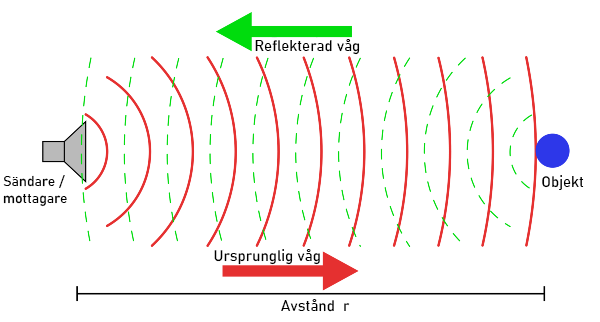
\includegraphics[scale=0.58]{dokumentation/projektrapport/IMAGES/Sonar.png}
    \caption{Avståndssensor. Avståndet räknas ut med: $r = (t * v_{ljud}) / 2$,\newline $t$ = tiden av högnivåsignalen från echo, $v_{ljud}$ = ljudets hastighet (343m/s).}
    \label{fig:Sonar}
\end{figure}
\newline\newline
Utöver detta tänder larmenheten en varningslampa så fort något närmar sig avståndssensorn. Avståndet för att tända lampan är dubbelt så långt som det konfigurerade värdet från centralenheten.
\newline\newline
Ifall larmenheten mottager ett meddelande från centralenheten hanteras det omedelbart med ett avbrott. Avbrottshanteraren för vidare meddelandet till en hanteringsfunktion beroende på vilken typ av meddelande det är. De meddelandetyper som hanteras är konfigureringsmeddelanden, meddelanden för att växla av/på larmet och pingmeddelanden. Ett konfigureringsmeddelande innehåller:\newline
\begin{itemize}
    \item En byte som bestämmer om larmet ska vara armed (se figur \ref{fig:module}).
    \item En byte som bestämmer om larmet ska slå larm/sluta slå larm direkt (se figur \ref{fig:cfg}).
    \item En byte som antingen kan:
    \begin{itemize}
        \item Ge en order att kalibrera sensorn efter de objekt som finns framför den i nuläget, detta sker när byten är noll.
        \item Ge ett bestämt avstånd som avståndssensorn ska konfigureras efter.
    \end{itemize}
\end{itemize}


När ett pingmeddelande är mottages skickas ett svarsmeddelande tillbaka. Dessutom sparar funktionen tidspunkten då larmenheten senast tog emot ett pingmeddelande. Eftersom larmenheten är den enda enheten i systemet som kan producera ett larm måste det finnas någon motåtgärd om larmenheten skulle kopplas ifrån systemet. Den motåtgärden består av att om larmenheten slutar tar emot ping-meddelanden från centralenheten i åtminstone en sekund larmar enheten automatiskt, dock är det värt att notera att centralenheten inte får ett meddelande om larmet är igång.


\subsection{Störenheten}
\label{sec:störenhet}
Störenheten har förmågan att skicka både korrekt strukturerade CAN-meddelanden eller slumpade datasträngar. Mängden data och frekvensen på meddelanden är inte konfigurerbara genom systemet utan måste föranpassas i koden. Detta anses acceptabelt då enheten är enkel och endast används när tester utförs på systemet. 


\subsection{Användning}
\label{sec:användning}
Programmet startar med en ''uppstartsfas'', där alla moduler kopplas till programmet automatiskt (se \ref{sec:centralenhetenDE}). Alla enheter är initialt icke-armerade, vilket betyder att de inte kan användas. För att armera modulen behövs USART-kommandon användas (se \ref{sec:centralenhetIO}). En användare som aldrig har använt programmet tidigare kan t.ex först skriva ''help'' för att se möjliga kommandon. Sedan kan användaren skriva ''printlist'' för att se vilka moduler är kopplade och deras ID. Slutligen kan användaren börja konfigurera eller armera/disarmera modulerna med ''arm/disarm [modul-ID]'' eller ''config [modul-ID]'', där [module-ID] är en av ID värdena från printlist. \\

När ett lokalt larm utlöses tänds en lampa, och på dörrenheten startas en timer. För att larma av innan ett globalt larm utlöses behöver användaren skriva in rätt pin-kod med knappsatsen. Om användaren skriver fel får den återkoppling via USART, och får ett nytt försök. Om det skrivs in mindre än fyra siffror kan användaren fortfarande börja om genom att trycka på knappen ''C'' (clear). \\

För att ansluta dörrar till en dörrenhet skall dörrsensorer kopplas till GPIOE 0-7, röda dioder till GPIOD 0-7 och gröna dioder till GPIOD 8-15. Om färre dörrar än åtta vill anslutas skall dessa anslutas till de lägra pinnarna. Sedan konfigureras antalet dörrar genom USART. Om t.ex två dörrar ska anslutas kopplas två dörresensorer till GPIOE 0-1, Två röda dioder kopplas till GPIOD 0-1 och två gröna dioder kopplas till GPIOD 8-9.
\iffalse
För att konkretisera en struktur som ett datorsystem underlättar det
ofta att rita en figur, till exempel ett blockschema, över systemet som
man tänker sig att implementera. I detta avsnitt beskriver ni
översiktligt systemet, lämpligen genom en (eller flera) figur(er). Se
till att hänvisa till figuren från texten och att använda en rubrik för
figuren. Eftersom systemet är ganska komplext behöver ni tänka igenom
vilken detaljrikedom systemöversikten ska ha; dels känner ni ännu inte
till detaljer eftersom konstruktionsarbetet inte påbörjats, dels skulle
inte alla detaljer få plats i en figur över systemet.

I och med att det finns ett grundsystem till vilket man kan lägga
kompletteringar behöver era val av kompletteringar beskrivas
översiktligt. Om ni avser att arbeta med egendefinierade kompletteringar
krävs en mer detaljerad beskrivning än om ni använder kompletteringar
som beskrivs i projektdirektivet.

Under projektets genomförande kommer ni att få anledning att revidera
figuren över systemet. Att ta fram den ultimata figuren över det
slutliga systemet är varken möjligt eller önskvärt under
planeringsfasen, utan det är framförallt processen med att ta fram
figuren som är viktig eftersom denna process hjälper gruppen att
fokusera tänkandet, att skapa gemensamma tekniska ramar och att rensa
bort (en del) tekniska oklarheter.
\fi
\newpage
%Resultat
\section{Resultat}
\label{sec:resultat}



Ett säkerhetssystem har utvecklats med hjälp av tre mikrokontroller och ett antal sensorer. En mikrokontroller fungerar som centralenhet, denna kommunicerar med två periferienheter som i sin tur har uppkopplade sensorer. Säkerhetssystemets funktionalitet har verifierats med ett flertal tester. Testerna utfördes på enhetsnivå och på systemet som helhet. De utförda testerna visar att systemet fungerar stabilt med pålitlig kommunikation mellan enheter och sensorer, samt att sensorerna  kan konfigureras så de agerar som önskat. Det övergripande testet, T17 (bilaga 17), som presenteras nedan visar översiktligt hela systemets funktionalitet, och mer detaljerade resultat finns under rubrikerna nedan. 



\subsection{Nätverkslagret}

CAN-nätverket som helhet fungerar väl. Meddelanden tas emot och hanteras korrekt. Prioritering av meddelanden fungerar utan krockar enligt test T5 (bilaga 5). Systemet klarar av när en störenhet skickar stora mängder data på CAN-bussen. I test T6 (bilaga 6) visas att systemet klarar av när en störenhet skickar ping-meddelanden konstant utan fördröjning så länge systemet skickar riktiga meddelanden mer sällan än 500 gånger per sekund.
\newline\newline
En störenhet som skickar slumpade meddelanden kan systemet inte hantera då viss data som skickas inte är av samma struktur som ett faktiskt meddelande.
Detta är en identifierad svaghet då CAN-protokollet är okrypterat. Dessa resultat visar att systemet uppfyller krav ett enligt \ref{sec:kravspec}. 

\subsection{Centralenheten}
Test T1 (bilaga 1) visar att centralenheten korrekt skapar en lista med alla uppkopplade enheters ID vid startup-fasen (se \ref{sec:centrallogik}). Detta test verifierar att systemet ansluter enheter modulärt, men visar även att kommunikationen mellan de anslutna enheterna fungerar som den ska. Enheterna svarar punktligt på alla ping-meddelanden som centralenheten skickar ut, och när en enhet blir frånkopplad går larmet. Dessa tester pekar på att systemet uppfyller krav ett, fem, och åtta enligt \ref{sec:kravspec}. 
\newline \newline 
T19 (bilaga 19) visar att information om enheternas konfigurationer lagras och uppdateras korrekt, enligt krav fem. Att meddelanden från enheter med okända ID-nummer ignoreras påvisas i T6 (bilaga 6). Därav uppfylls krav två enligt \ref{sec:kravspec}. 
\newline \newline
Centralenhetens IO-funktioner har förmågan att utföra samtliga kommandon begärda från USART. Dessa inmatningar används av centralenheten för att konfigurera periferienheterna eller begära information om systemet. Denna funktionalitet visades i T15 (bilaga 15). Knappsatsen brukades för att stänga av ett aktivt larm, och detta fungerade vid upprepade försök i test T10 (bilaga 10). Dessa tester visar att krav tre är uppfyllt enligt \ref{sec:kravspec}.

\subsection{Dörrenheten}
%krävs åter igen mycket tester 
%bevisa att 8 dörrar stöds?
Test T12 (bilaga 12) visar att dörrenheten kan larma lokalt. Testet visar också att en dörr kan tända en diod för att markera att den är ställd till att inte larma. Test T13 (bilaga 13) visar på att dörrar kan ställas att larma eller inte från centralenheten. Slutligen visar test T15 (bilaga 15) en större överblick på att funktionaliteten är korrekt. Där demonstreras att tidsgränser går att konfigurera och att enheten kan utlösa det globala larmet. Dessa resultat visar att dörrenheten uppfyller krav fyra och sex enligt \ref{sec:kravspec}.


\subsection{Larmenheten}
Avståndssensorn och vibrationssensorn är funktionella. Avståndssensorn larmar lokalt när något kommer närmre än ett konfigurerat avstånd, vilket visas i test T2 (bilaga 2). T4 (bilaga 4) visar att det globala larmet aktiveras korrekt när avståndet är under ett andra tröskelvärde. Systemtestet T17 (bilaga 17) visar att larmenheten kan konfigureras av centralenheten eller själv kalibrera larmavståndet på order från centralenheten. Resultaten ovan visar att larmenheten uppfyller krav fyra och sex enligt \ref{sec:kravspec}.
\newline\newline
Test T7 (bilaga 7) visar att om inget pingmeddelande från centralenheten är mottaget inom önskat tidsintervall utlöses larmet. Det globala larmet kan även stängas av och på från centralenheten. Detta visas i test T8 (bilaga 8). Dessa resultat visar att larmenheten uppfyller krav fem och sju enligt \ref{sec:kravspec}.
\newline\newline
Det utfördes även ett test på avståndssensorns felmarginal, T4 (bilaga 4), vilket visade att det uppmätta avståndet var mycket konsekvent och hade en felmarginal på under en centimeter.

\newpage
%Slutsatser
\section{Diskussion}
\label{sec:diskussion}
%Detta avsnitt innehåller en sammanfattning av konstruktionen och en diskussion av resultatet. Om det
%är möjligt, dra slutsatser av ert projekt och identifiera förbättringsmöjligheter
%(vilka kan vara användbara för en beställare).
Slutresultatet uppnår de krav som sattes på arbetet, se \ref{sec:kravspec}. Larmenheten, dörrenheten och centralenheten arbetar tillsammans för att uppfylla de krav som ställdes för ett fungerande lås- och larmsystem. Centralenheten övervakar enheternas status regelbundet. Vid otillåtet intrång skickar dörrlarmet respektive rörelselarmet en signal att larma. Kommunikationen mellan enheterna sker på ett konsekvent sätt med det designade CAN-protokollet. Centralenheten lägger till enheter på ett modulärt sätt, enligt krav åtta. Däremot är det inte perfekt då ID-nummer inte delas ut dynamiskt utan är hårdkodade hos enheterna. Trots detta är systemet på bra väg att vara modulärt.
\newline \newline
Utöver grundsystemet utfördes också två utökningar av rörelselarmet. Rörelselarmet larmar lokalt inom ett visst distansintervall från rörelesesensoren och sedan globalt då intervallet överskrids. Sedan har dessutom en distinkt larmsignal framställts.
\subsection{Struktur}
\label{sec:structfunc}
Under projektets utveckling har det lagts en viss vikt på att generalisera hanteringen av modultyperna. Denna generalisering underlättas mest av modul-structen som beskrivs i sektion \ref{sec:centralenhetDL}. Att använda en gemensam datatyp för modultyperna gör det enklare att samla alla enheters information på samma ställe, i en sorts lista. Listan med enheter skulle kunna filtreras, sorteras och sökas i, vilket är en stor fördel. Om systemet skulle utökas blir dessa funktioner praktiska, mest för användaren. 
\newline \newline 
När information om en specifik modul ska uppdateras är användingen av en lista lämplig; listan söks igenom, och enhetens modul-struct uppdateras. Detta gör det möjligt för centralenheten att lagra aktuell information om alla enheter, enligt krav två i \ref{sec:kravspec}. Att samtlig information om enheterna lagras på samma plats underlättar också för utvecklare. En ny modultyp skulle kunna läggas till i systemet utan att behöva ändra på projektets struktur.
\newline \newline
Denna struktur gör dock systemet mer komplicerat, och detta kan ha negativa effekter. En komplex struktur gör det svårare att identifiera misstag eller logiska fel. Därför kan systemets säkerhet och funktionalitet bli svårare att verifiera. Men om ett komplext systems kod är en välskriven och verifierad bas för systemet främjar detta framtida utveckling. Då underlättar den befintliga koden förståelse och vidareutveckling av systemet.
\newline \newline 
En stor förbättring när det gäller generalisering skulle vara att skapa en universell modultyp för sensorer. I det nuvarande läget har larmenheten hand om vibrationssensorn och rörelsesensorn, medan dörrenheten har hand om flera magnetkontakter (eller dörrsensorer). Om en sensormodul implementeras skulle den kunna hantera alla sensorer som tidigare var kopplade till larmenheten och dörrenheten samtidigt, och utöver det skulle den kunna hantera ännu fler sensortyper. Modulens datahantering kan implementeras som centralenhetens: en generell struct för sensorer finns, och information lagras om dessa i modulens minne. Alla funktioner som är specifika för att konfigurera samt avläsa sensorerna skulle då kunna skrivas separat, och importeras av modulen som ett programbibliotek. Detta underlättar processen att lägga till en ny sensortyp.

\subsection{Funktionalitet och IO} % inte färdig
\label{sec:funktionalitet}

%Utvärdera hur enkelt det är att använda programmet, vad man kan göra. 

%USART skulle kunna skriva ut automatiska status-uppdateringar vid konfiguration ändringar och liknande. I nu-fallet om en modul konfigureras så kollas det om inmatningen fungerar, och i så fall antas att konfigureringen sker korrekt. Istället skulle funktionerna kunna skriva ut de konfigurerade enheternas nya status efter ändringen för att tydligare visa vad som har hänt. \\

%Vissa kommandon till programmet skulle kunna förtydligas och utökas. Help kommandot ger en kort beskrivning av vad varje kommando gör, vilket är korrekt. En addition skulle vara att göra det möjligt att skriva "Help [kommando]" för att ge extra information och detaljer om varje kommando. Utan detta behöver användaren ha tillgång till projektrapporten för att fullt förstå hur ett kommando fungerar.

%Diskutera användarens möjlighet att påverka systemet och systemets möjlighet att presentera information och visa resultatet av användarens påverkan.

Funktionellt skall systemet tillåta användaren att påverka systemet samt presentera information och visa resultatet av användarens påverkan. Användaren har två olika sätt att interagera med systemet: genom USART-kommandon och genom en knappsats. Detta tillåter att alla perifirienheter kan konfigureras fullständigt vilket täcker kraven på funktionalitet. \\

Systemets förmåga att ge användaren feedback är i nuläget begränsad. Centralenheten begär inte information från periferienheterna när de konfigureras. Därmed kommer ingen automatiskt utdata om ändringarnas effekt. Den lokala statusen kan fortfarande ses manuellt med USART-kommandon, men den kan vara olika från statusen på periferienheterna. Det uppnår kraven på funktionalitet, men operationen kan förenklas och optimeras. \\ 

Projektets moduler läggs nu till automatiskt vid uppstart, förutsatt att alla periferienheter har sina ID-nummer fördefienerade. Denna process är dock inte helt konfigurationsfri; användaren behöver defienera alla periferienheters ID i respektive källkod innan koden laddas. Detta skulle kunna förbättras och en utveckling av systemet är därför att implementera automatisk ID-utdelning för att göra det mer användarvänligt. Vid uppstart skulle centralenheten då dela ut ett unikt ID-nummer till alla enheter. Detta skulle göra systemet helt konfigurationsfritt och användaren skulle bara behöva koppla in de nödvändiga enheterna och trycka ''start''. 
\newline \newline 
Om den automatiska ID-utdelningen implementeras kan man anse att systemet är fullständigt modulärt. Det kan då kopplas flera dörr- och larmenheter till systemet, och det antalet moduler som kan vara kopplade samtidigt kan ändras. 
Ett icke-modulärt system, som har ett fast antal enheter, kan vara enklare att använda och det kan också vara säkrare. Att inte ha en uppstartfas som lägger till alla tillkopplade enheter minimerar risken att en oönskad modul kan läggas till i systemet, och att ändra på systemet kanske  blir svårare eftersom CAN-systemet inte skulle vara lika generellt. Den negativa sidan med ett sådant system är så klart att det inte är modulärt.

\subsection{Delsystemen}
% Nätverkslagret
Nätverkslagret tillfredsställer i slutändan projektets krav för kommunikation. Enheterna kan kommunicera genom en gemensam CAN-buss där meddelandekollisioner löses utav det skapade CAN-biblioteket. Genom prestandatester som beskrivs i \ref{sec:resultat} säkerställs, med hög sannolikhet, att nätverkslagret är robust för sabotage och tekniska fel. Däremot hade förbättringar kunnats göra som exempelvis att kryptera datan som skickas över bussen. Detta nämns mer i \ref{sec:sakerhet}. En annan förbättring hade kunnat vara att inkludera ett så kallat \textit{ACK-fält} i CAN-ramen. Det denna gör beskrivs i \ref{sec:can}. Att ha detta fält hade kunnat säkerställa att meddelanden som läggs ut på bussen faktiskt når den avsedda mottagaren. Då hade potentiellt snabbheten hos CAN-meddelandena försämrats då mer information måste utbytas. Däremot bör denna prestandaförändring vara oväsentlig.
\newline\newline
%Larmenheten
Larmenheten hanterar dess uppgifter enligt ställda krav. Avbrott prioriteras och utför ändringar omedelbart utan att påverka prestandan av sensorerna. En potentiell utökning av antalet möjliga sensorer av samma typ skulle gynna systemet i hög grad. Det skulle kräva en omstrukturering av GPIO-pinnarna samt att alla sensorfunktioner i programlogiken måste modifieras för att hantera fler än bara en modul i taget. Det skulle resultera i en drastisk minskning av antal MD407-kort för fullständiga system, med en potentiellt minimal försämring av prestanda. 
%Dörrenheten
\newline\newline
Dörrenheten är satt att hantera max åtta dörrar. Ett MD407-kort har 32 GPIO-pinnar. Varje dörr kräver tre, en för dörrsensorn och två för dioderna. Den fysiska begränsningen är alltså tio dörrar. Valet att ha max åtta dörrar gjordes med anledning av enkelhet för användaren. På MD407-kortet är pinnarna uppdelade i fyra grupper, pinnarna 0-7 och pinnarna 8-15 för både GPIOE och GPIOD, se bild \ref{fig:doorgpio}. 
Det finns alltså plats för två dörrsensorer och fyra dioder till på GPIOE 8-15. Nackdelen med det blir att användaren som skall koppla upp systemet får en mindre intuitiv och rörigare uppkoppling då en GPIO-port kommer vara både utport och inport, alltså ha både dörrsensorer och dioder. Därav valdes åtta dörrar.
\begin{figure}[h]
    \centering
    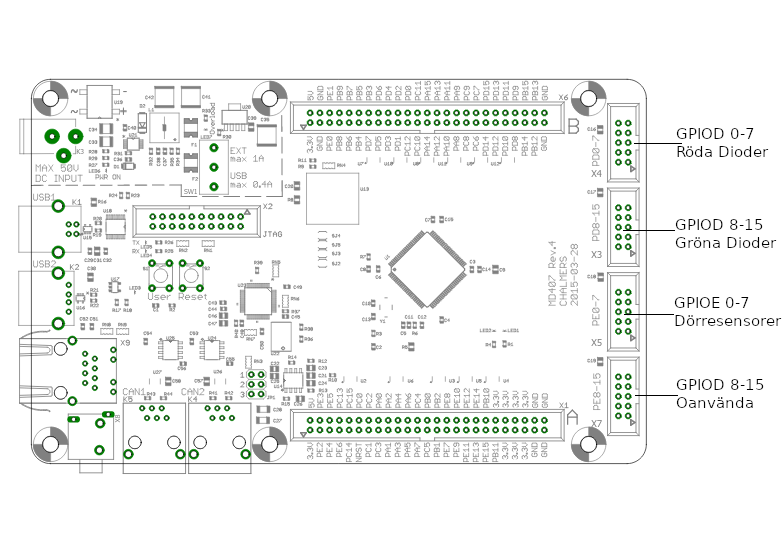
\includegraphics[scale=0.55]{dokumentation/projektrapport/IMAGES/doorgpio.png}
    \caption{GPIO-pinnarnas användning på dörrenheten\cite{md407}}
    \label{fig:doorgpio}
\end{figure}
\subsection{Säkerhet}
\label{sec:sakerhet}
Vissa åtgärder togs för att förbättra säkerheten. Alla funktioner i programmet kontrollerar sin indata innan något görs med den för att säkerställa att inget oförutsägbart sker i programmet. Utöver det kan moduler bara läggas till i modullistan under uppstarts-fasen, och efter det ignoreras alla mottagna meddelanden med okända nodID-nummer. Detta ger en viss säkerhet mot intrång i systemet, men garanterar inte detta till 100 \%. \newline \newline
I det nuvarande läget finns det många möjligheter att utveckla systemets säkerhet. Projektets implementation av CAN är funktionellt, men inte säkert. De säkerhetsåtgärder som vidtogs för modullistan nämns i stycket ovan, men skyddet som uppförs av dessa kan enkelt kringgås. Om en enhet ansluts till nätverket kan den skicka meddelanden i en annan enhets namn. Allt som krävs är att den externa enheten skickar ett meddelande med samma ''nodeid'' som en modul i modullistan. Denna enhet kan antingen gissa sig fram till detta ID, eller extrahera informationen ur ett CAN-meddelande från bussen. \newline \newline
Anledningen varför alla anslutna enheter kan läsa informationen på bussen är för att meddelandena inte är krypterade. Att implementera kryptering i kommunikationssystemet skulle vara ett stort steg för systemets säkerhet. Det skulle göra det betydligt svårare för en enhet att skapa meddelanden som följer projektets kommunikationsstandard, förutsatt att enheten inte har tillgång till den informationen. Attacker där en enhet kopierar ett redan krypterat meddelande och skickar det igen är svårare att hantera. Det finns lösningar till det problemet, men de är avancerade.
\newline \newline
När det gäller IO kan säkerheten utvecklas. Ett användarsystem för USART med olika behörighetsnivåer skulle kunna implementeras. Där skulle en administratör exempelvis kunna hantera vilka pin-koder som larmar av, och lägga till nya användare på en lägre eller lika hög behörighetsnivå.
\subsection{Utvärdering av tester}
De flesta av de utförda testerna var funktionella. Alltså testade de att en viss funktion fungerade korrekt. De minsta möjliga funktionerna testades först. När tester på mer omfattande funktioner gjordes var det då redan säkerställt att eventuella fel inte låg på underliggande kod. Det förenklade felsökningen och utvecklingen. 
\newline\newline
Endast en handfull mängd prestationstester utfördes och de var relaterad till störenheten, CAN-bussen och rörelsesensorn. Om fler prestationstest hade utförts hade systemets gränser varit bättre definierade. Detta hade förtydligat förbättringmöjligheter och säljpunkter för systemet.
Ett säkerhetstest med en tredje part hade kunnat utföras för att värdera säkerheten och upptäcka svagheter i systemet. Det har dock inte utförts i brist av tid.
\newline\newline
För kod skrevs tester för att bevisa korrekt funktionalitet. De testerna skrevs efter att given icke-trivial funktion var klar. Om testerna hade gjorts i förväg hade de varit användbara verktyg för utvecklingen. Det är också oklart hur mycket tid som hade sparats när man räknar med skapandet av testerna. Dessutom låg svårigheten generellt inte i mjukvaran utan i hårdvaran som testades med funktionalitetstester. 
\label{sec:utvärderingtest}
%Resultatet i förhållande till krav som beskrivs i planering och kanske syfte? 
%(Hur bra tester gjordes kanske är värt att diskutera)

\newpage
\section{Slutsats}
\label{sec:slutsatser}
Arbetet att utveckla ett säkerhetssytem med mikrokontrollern MD407 anses vara lyckat. Det skapade säkerhetssytemet uppfyller de krav som ställts i \ref{sec:kravspec}. Systemet är dessutom utökat med en svårmissad larmsignal och förmågan för larmenheten att larma lokalt eller globalt beroende på hur nära något är. Systemet levererades i tid.
\newline\newline
Systemet är modulärt på det sättet att inläggning av enheter vid uppstart sker automatiskt vilket är i enlighet med krav åtta (\ref{sec:kravspec}). Enheternas identifikationsnummer måste dock definieras av användaren i koden. Att lägga till automatisk ID-utdelning vid uppstart skulle vara en bra vidareutveckling av systemet. En gemensam datatyp brukas även för alla enheter i centralenheten. Detta gör det möjligt att samla deras information på samma ställe och underlättar även framtida enhetsutökningar. Enhetslistan kan sökas igenom och uppdateras. Likaså har CAN-funktionerna generaliserats, utom de som tolkar meddelandena då det för dessa ibland är nödvändigt att integrera dem med enhetens egna logik.
\newline\newline
Testningen utfördes först på mindre funktioner, varpå större och större stycken testades tills dess att hela systemet testats. Mer tester hade kunnat göras och mer vidareutvecklingsmöjligheter hade då kunnat hittas. Tester kunde även ha konstruerats i förväg som gjort det möjligt att spara mer tid.
\newline\newline
All skriven kod är välkommenterad och följer samma kodkonvention och systemet är tämligen modulärt. Allt det här underlättar och möjliggör för ytterligare utvecklingar av systemet.





\newpage

\bibliographystyle{IEEEtran} 
\bibliography{referenser}
 
\newpage

\LARGE {\centering {\section*{Bilagor}}}
\addcontentsline{toc}{section}{Bilagor}

\label{sec:bilagor}

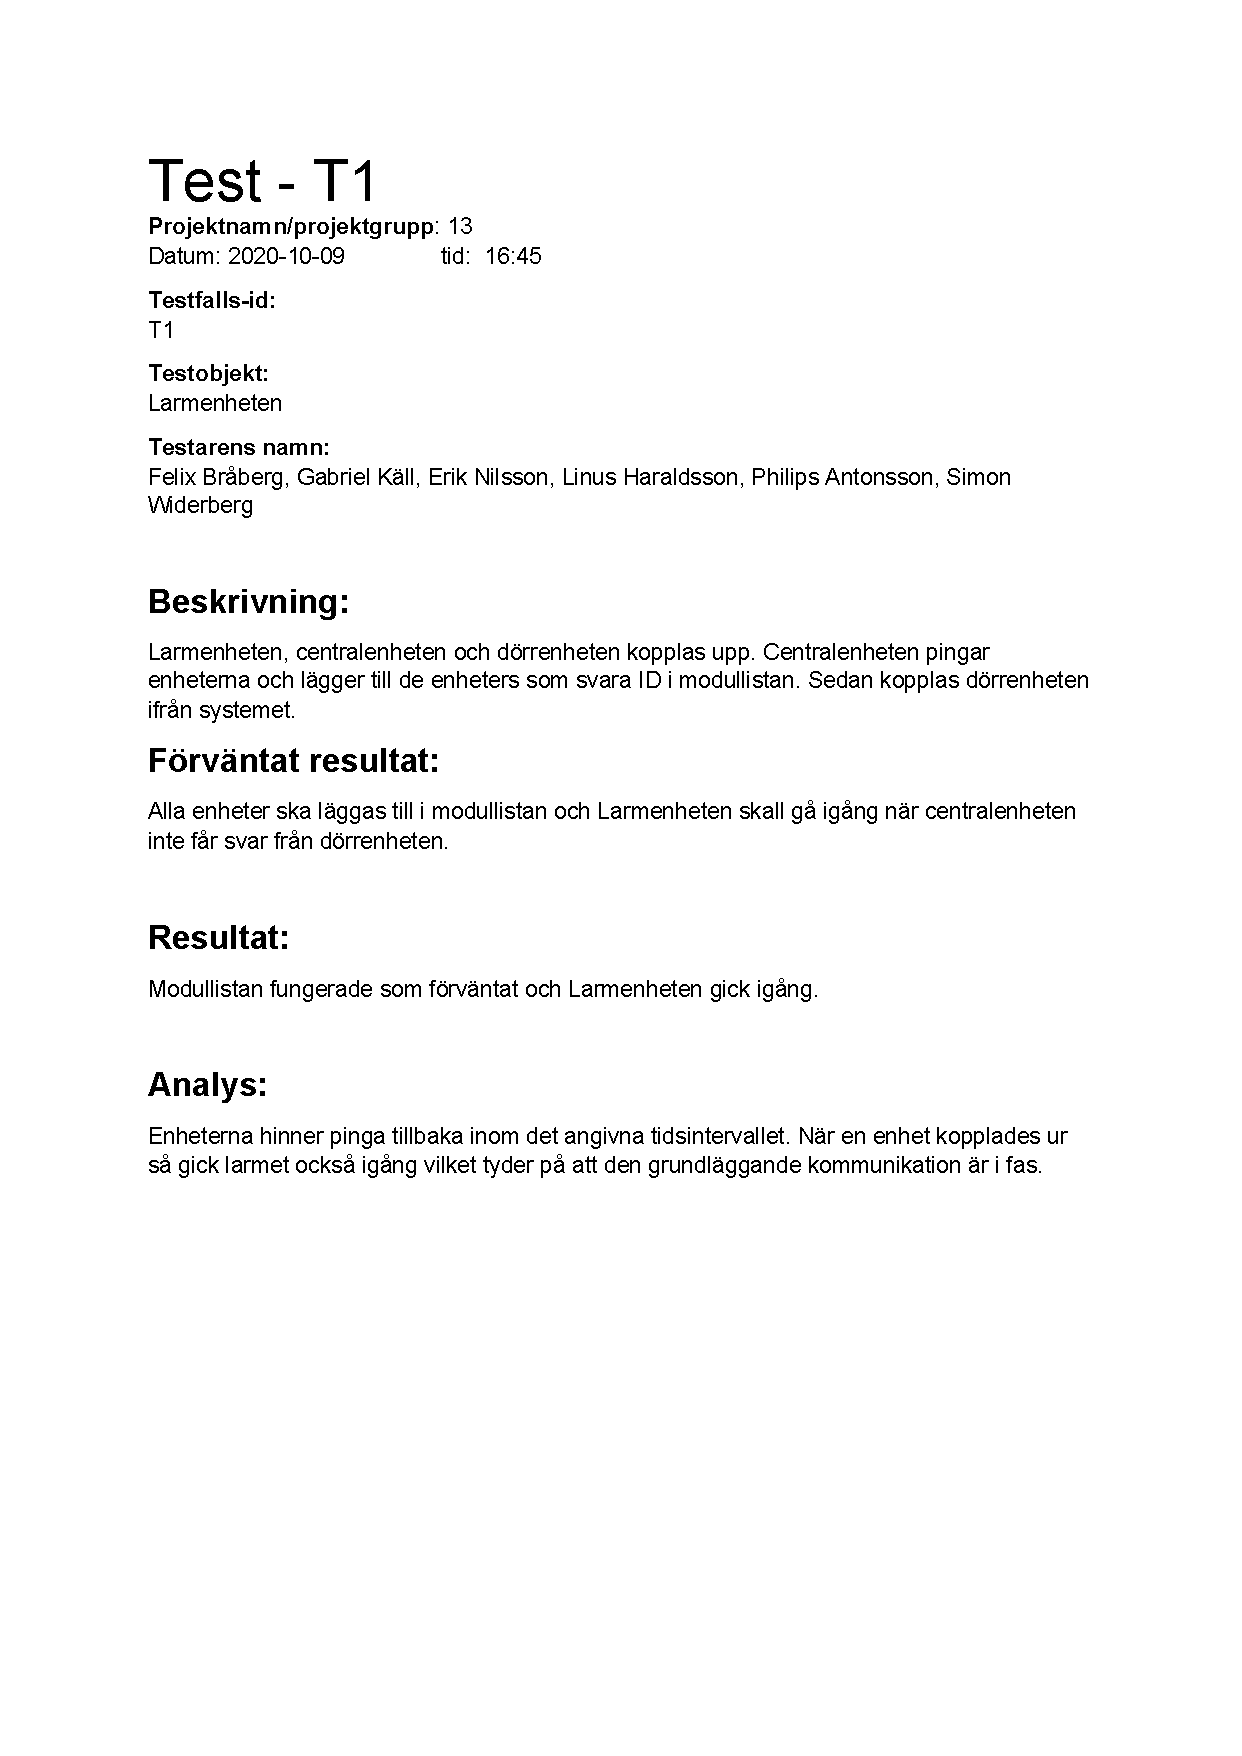
\includepdf{dokumentation/projektrapport/TESTS/Larmenhet_Test-T1.pdf}
\label{bil:T1}

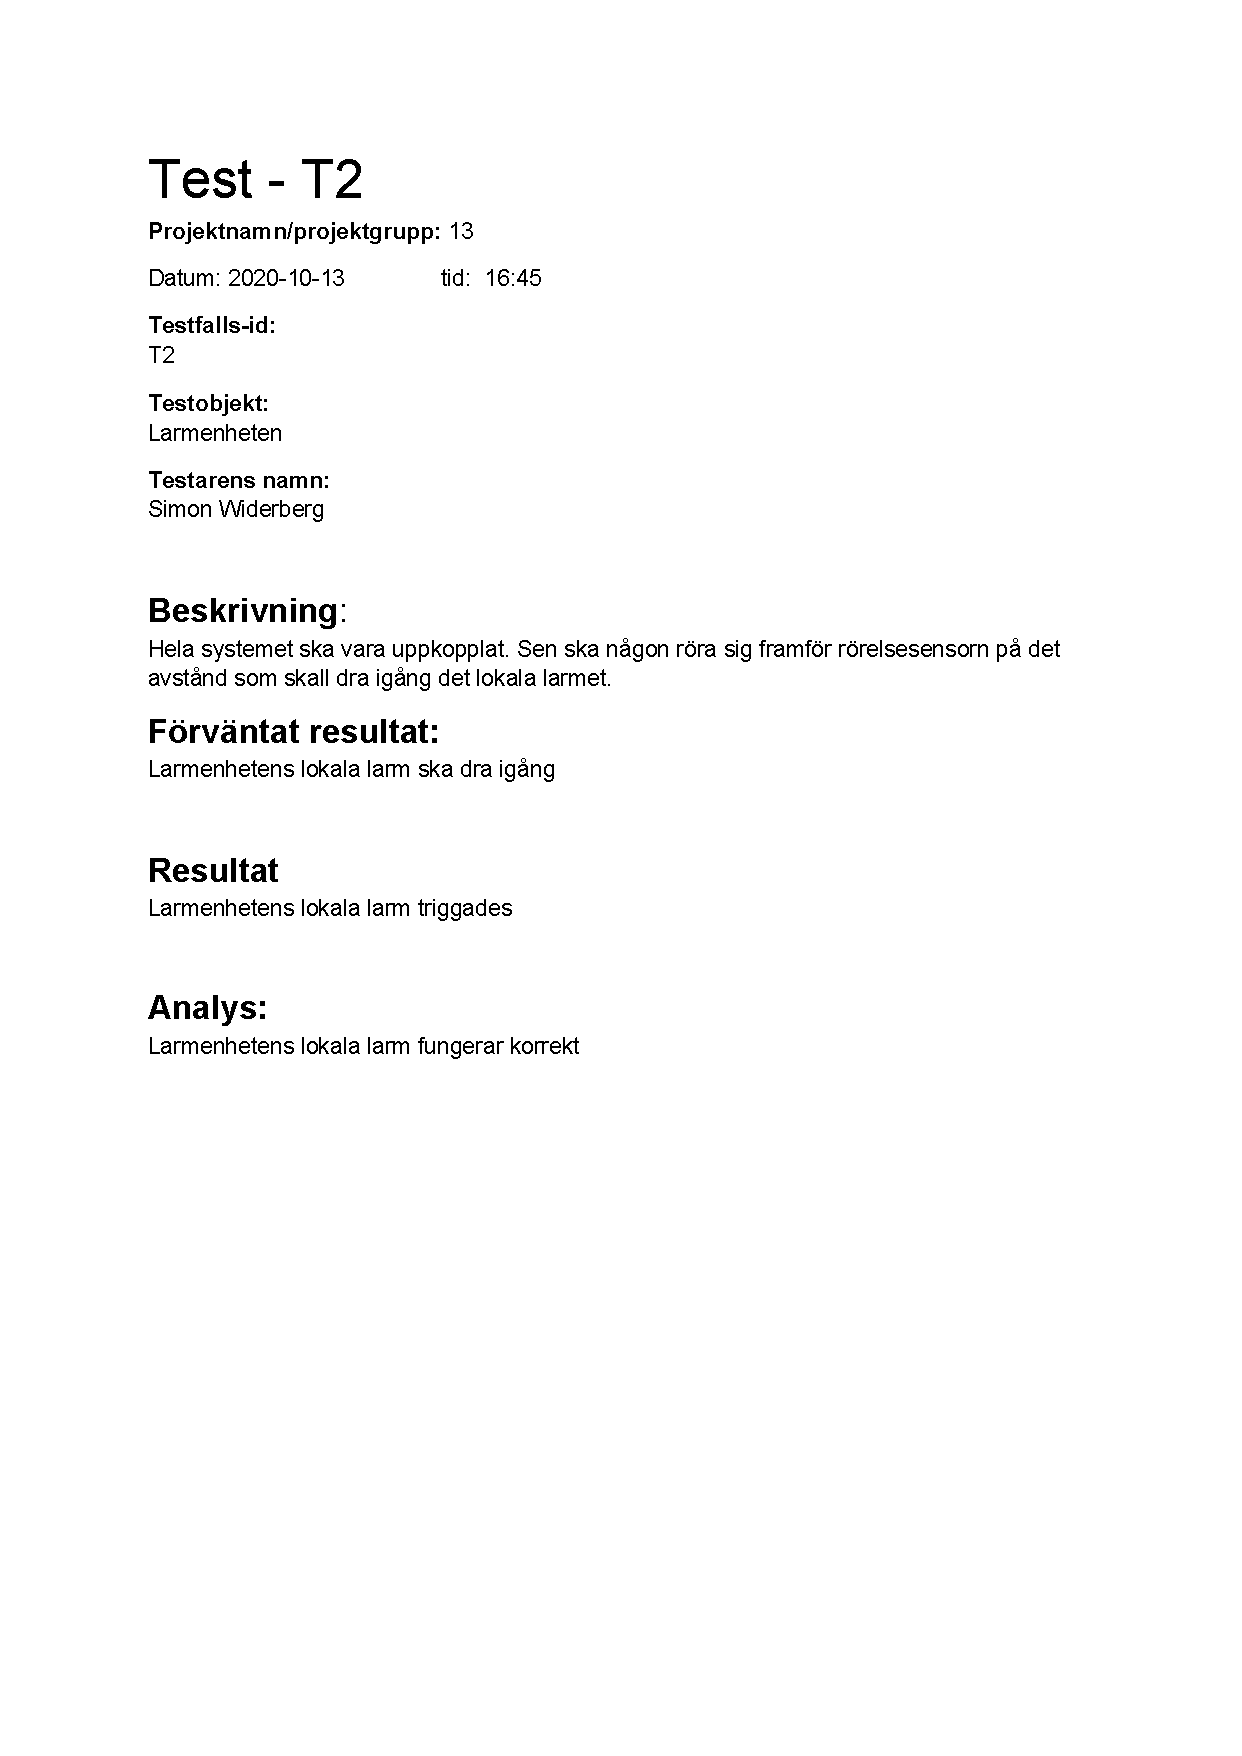
\includepdf{dokumentation/projektrapport/TESTS/Larmenhet_Test-T2.pdf}
\label{bil:T2}

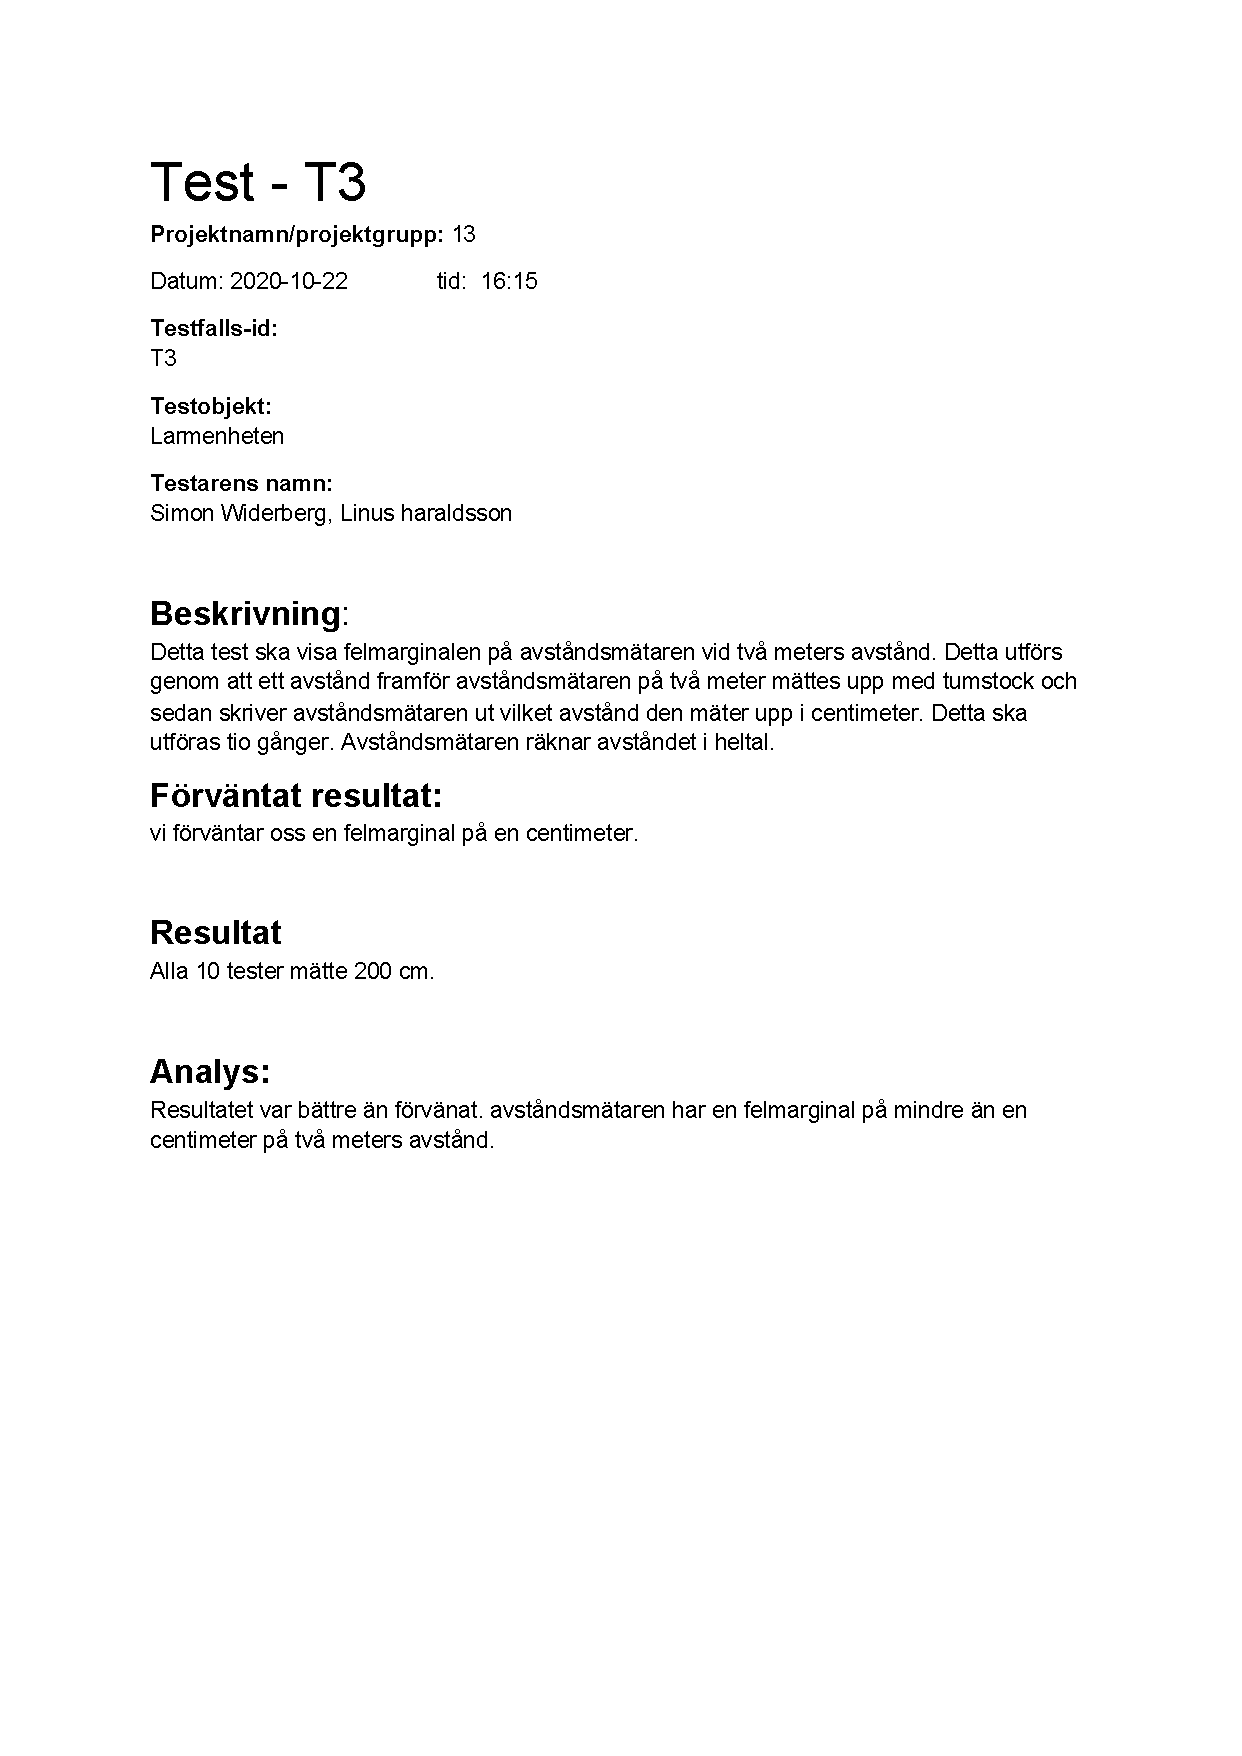
\includepdf{dokumentation/projektrapport/TESTS/Larmenhet_prestanda_Test-T3.pdf}
\label{bil:T3}

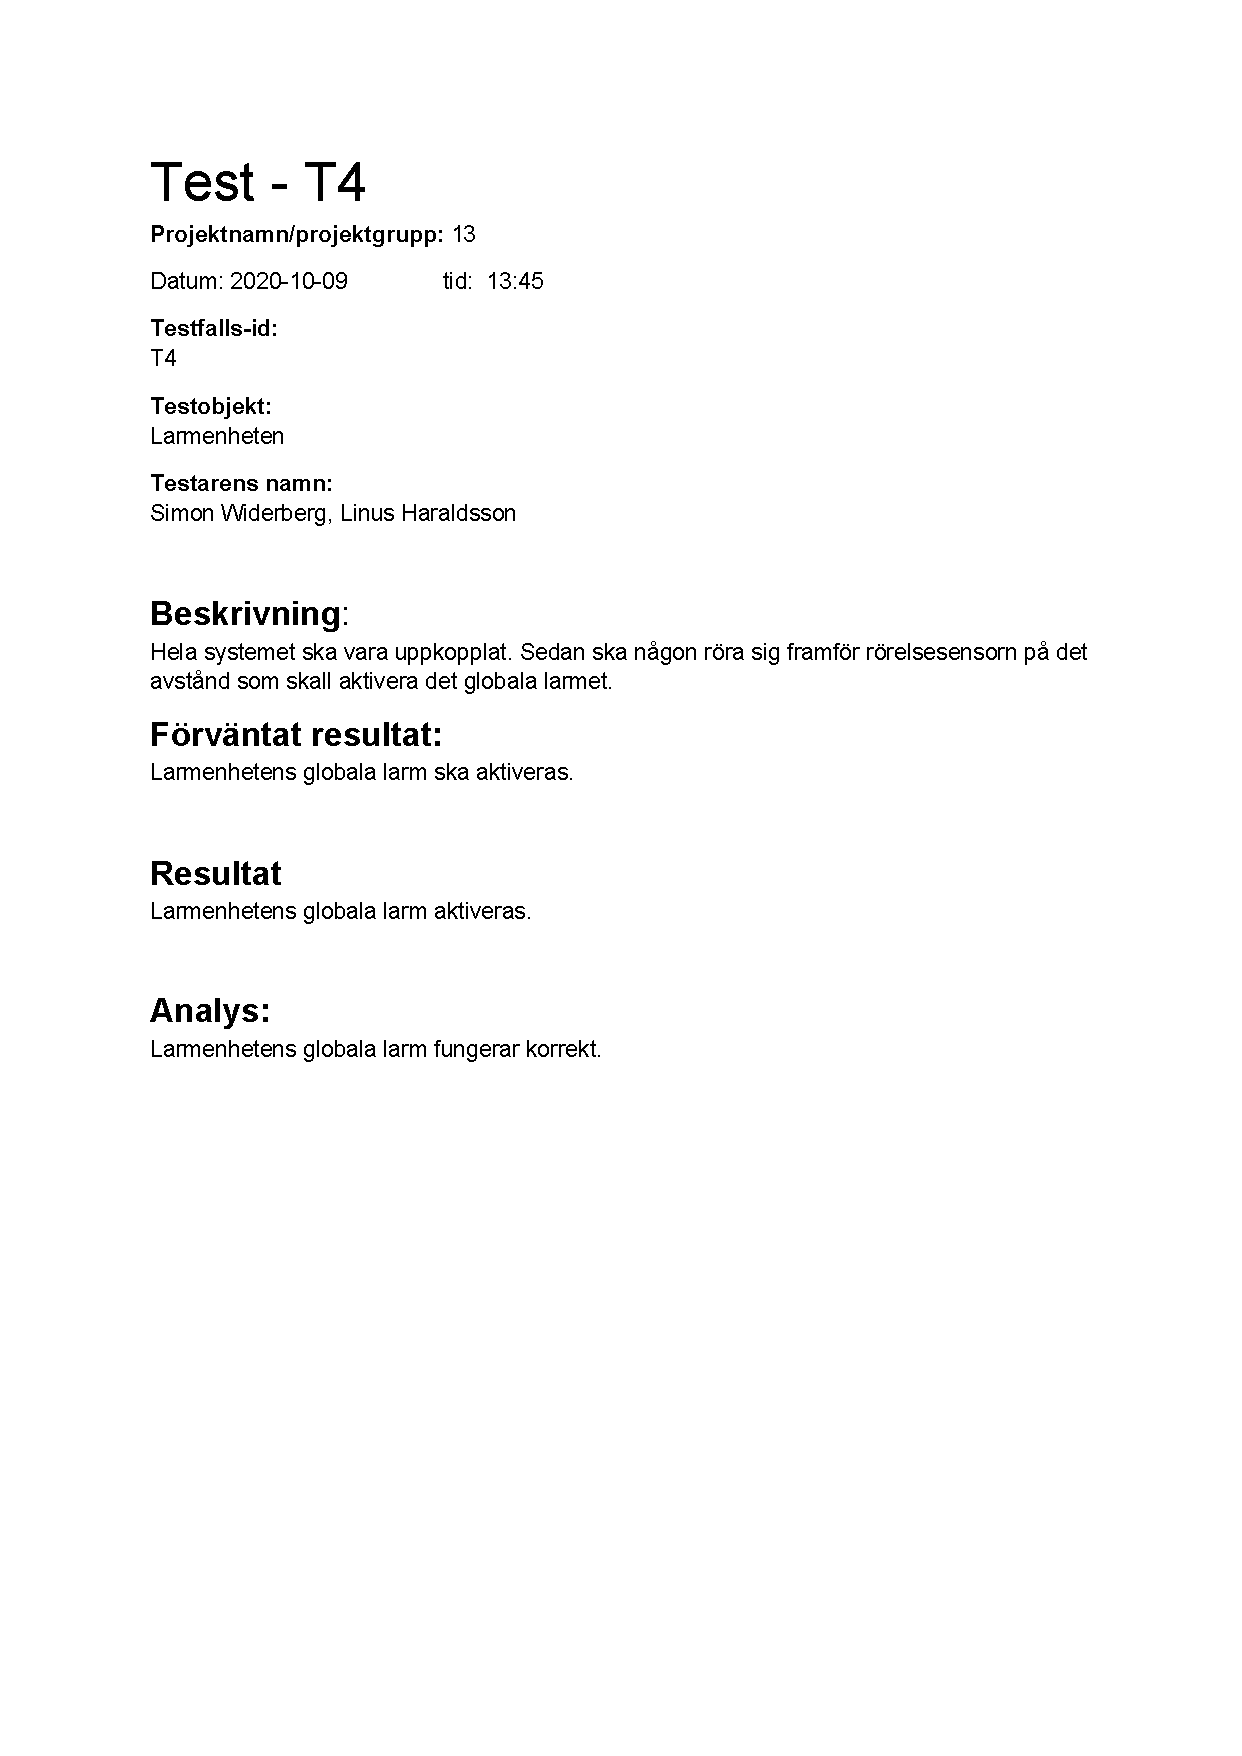
\includepdf{dokumentation/projektrapport/TESTS/Larmenhet_Test-T4.pdf}
\label{bil:T4}

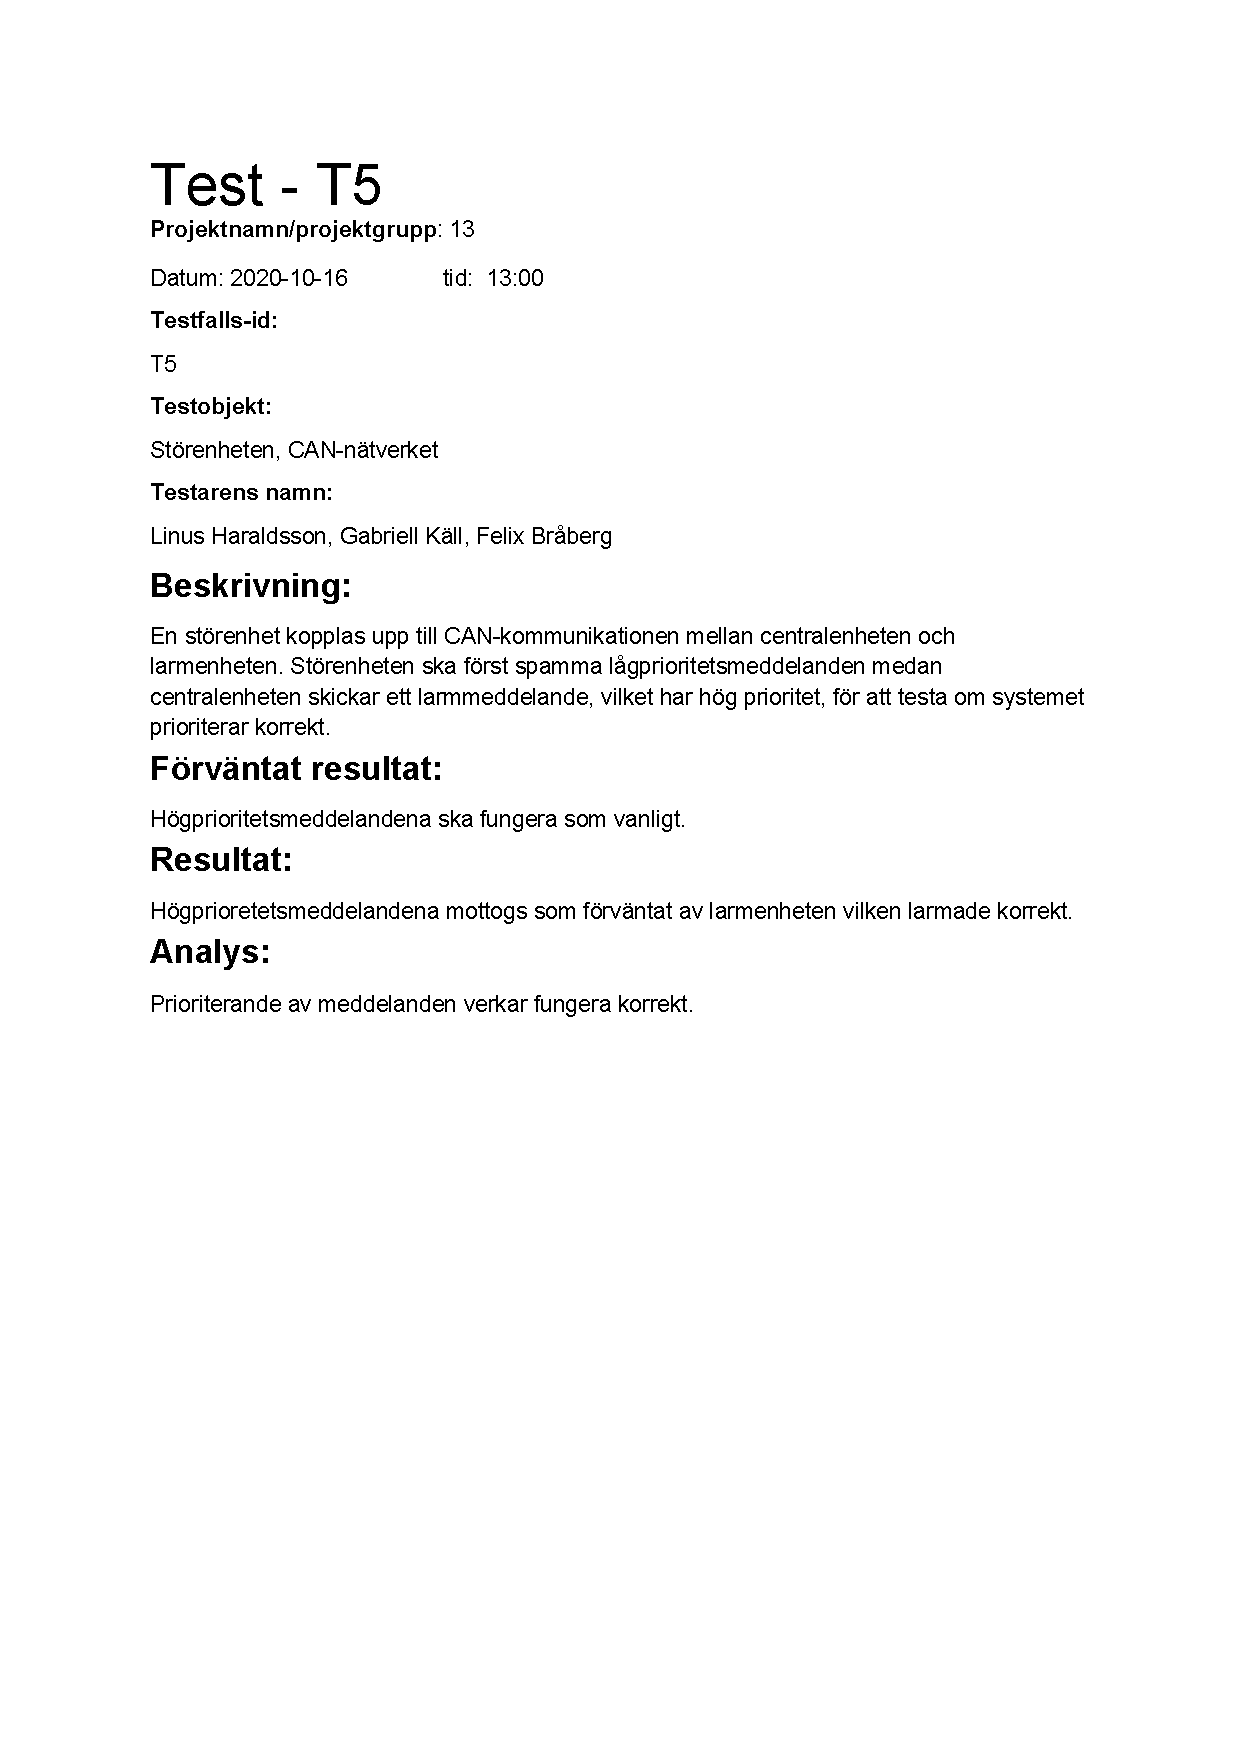
\includepdf{dokumentation/projektrapport/TESTS/Prioritet_Test-T5.pdf}
\label{bil:T5}

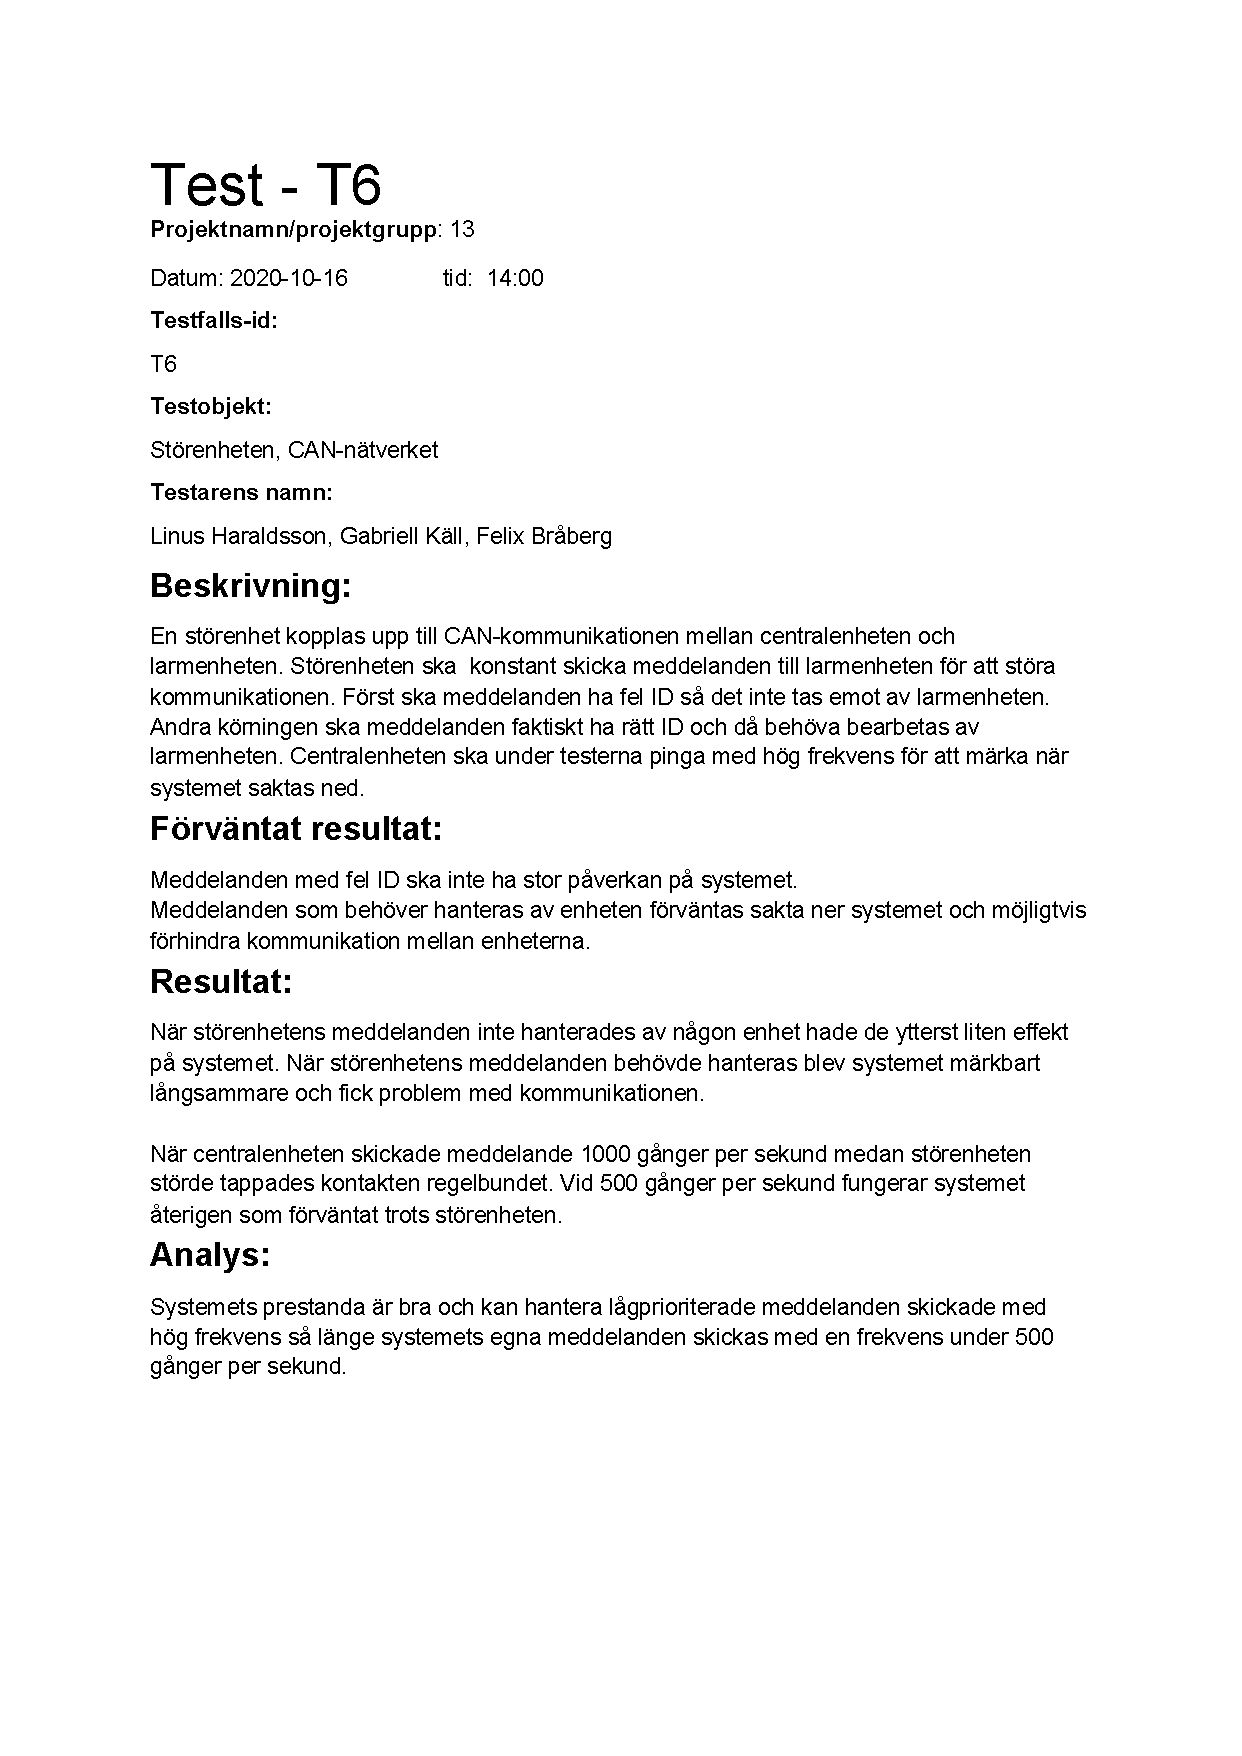
\includepdf{dokumentation/projektrapport/TESTS/Storenhet_Test-T6.pdf}
\label{bil:T6}

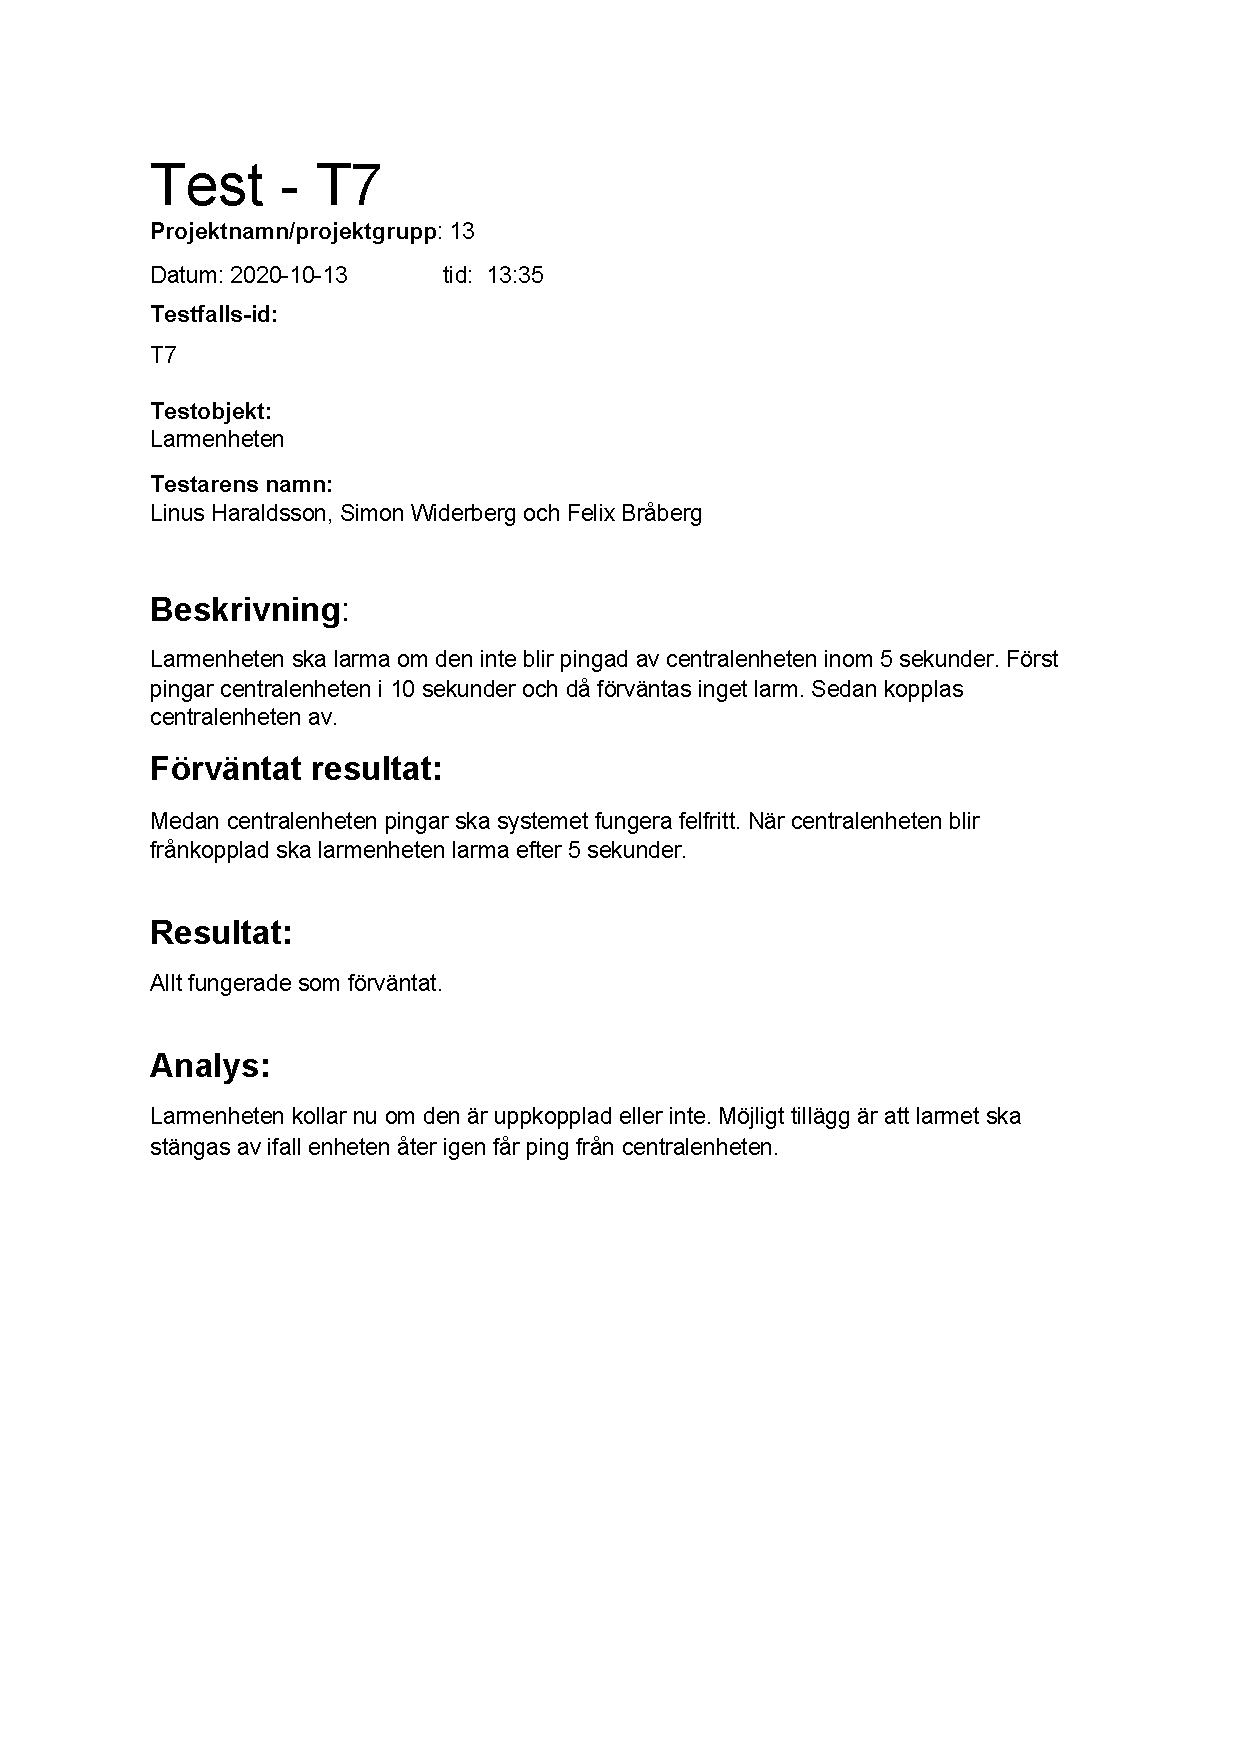
\includepdf{dokumentation/projektrapport/TESTS/Larmenhet_Test-T7.pdf}
\label{bil:T7}

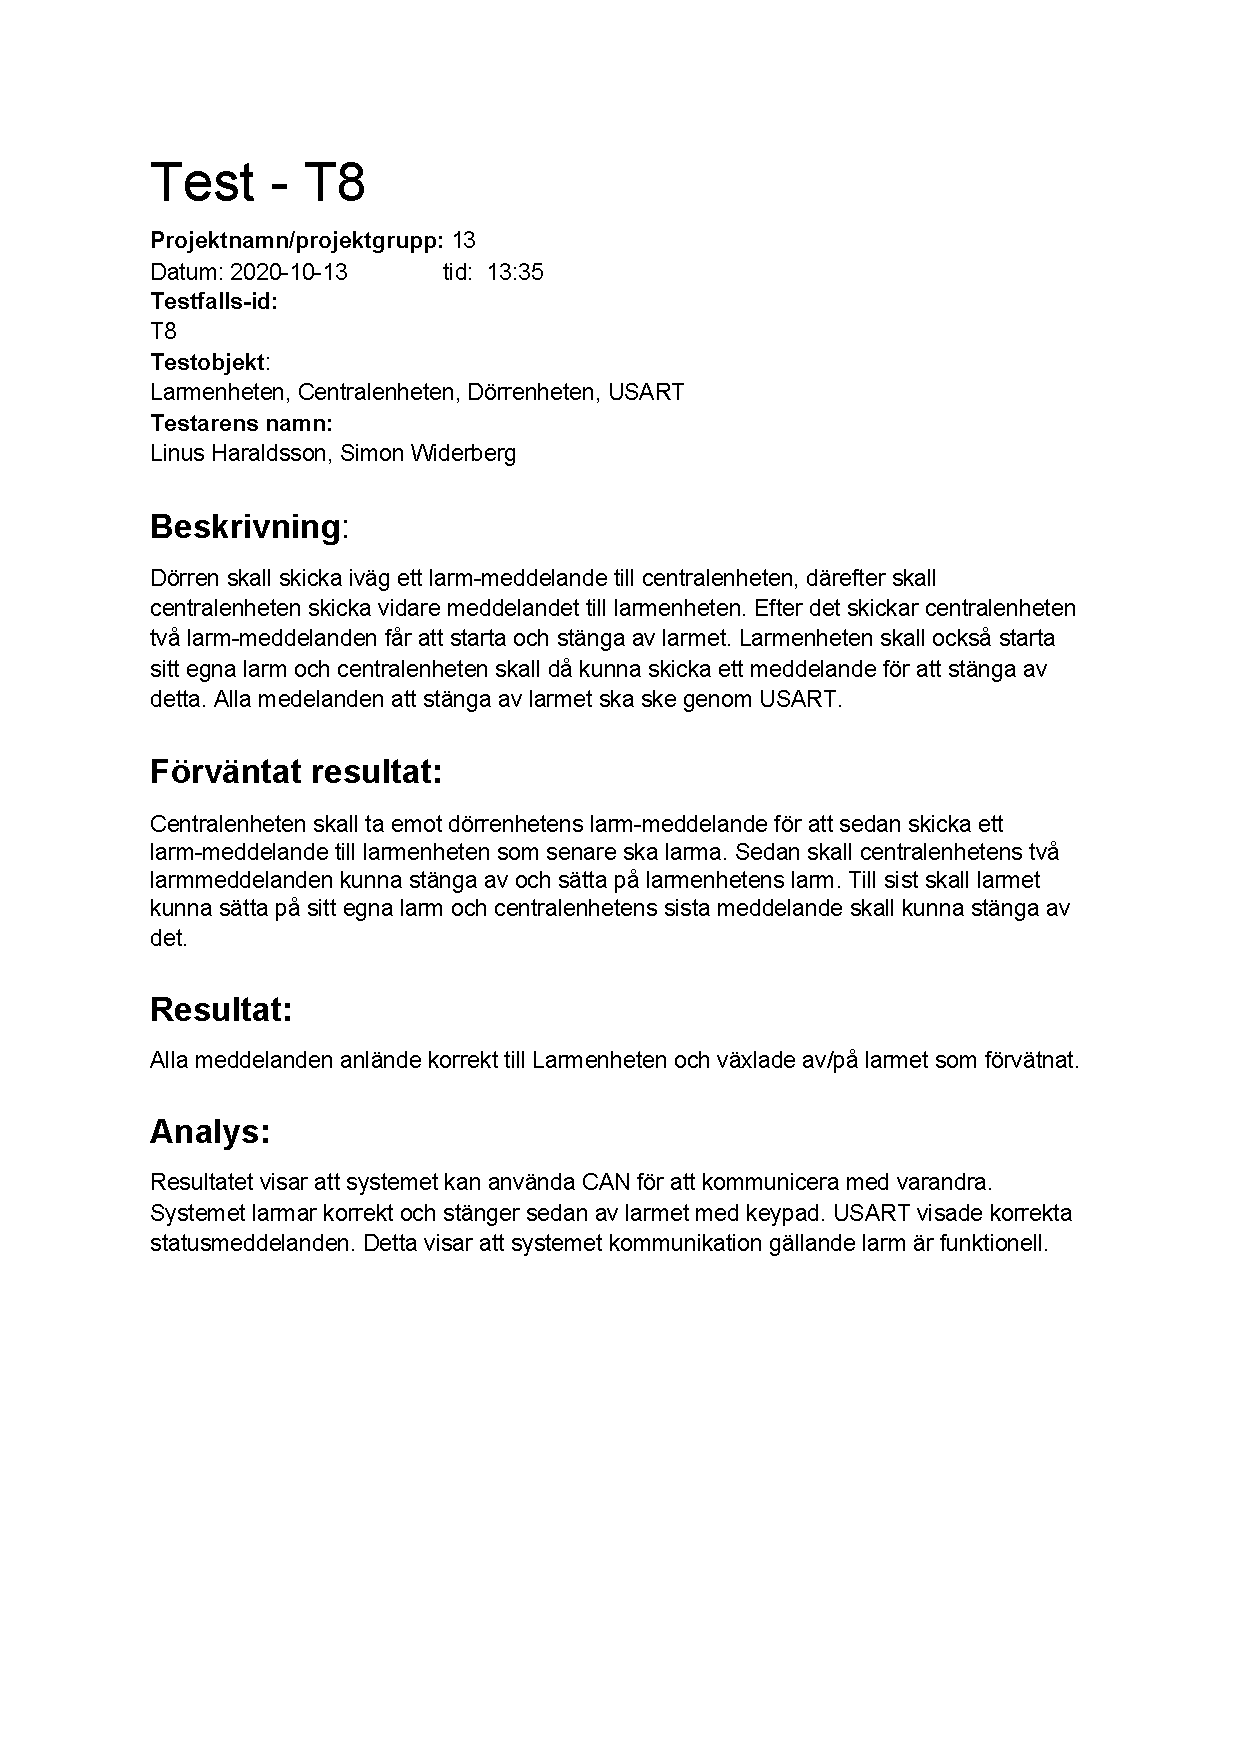
\includepdf{dokumentation/projektrapport/TESTS/Larm_och_systemtest-T8.pdf}
\label{bil:T8}

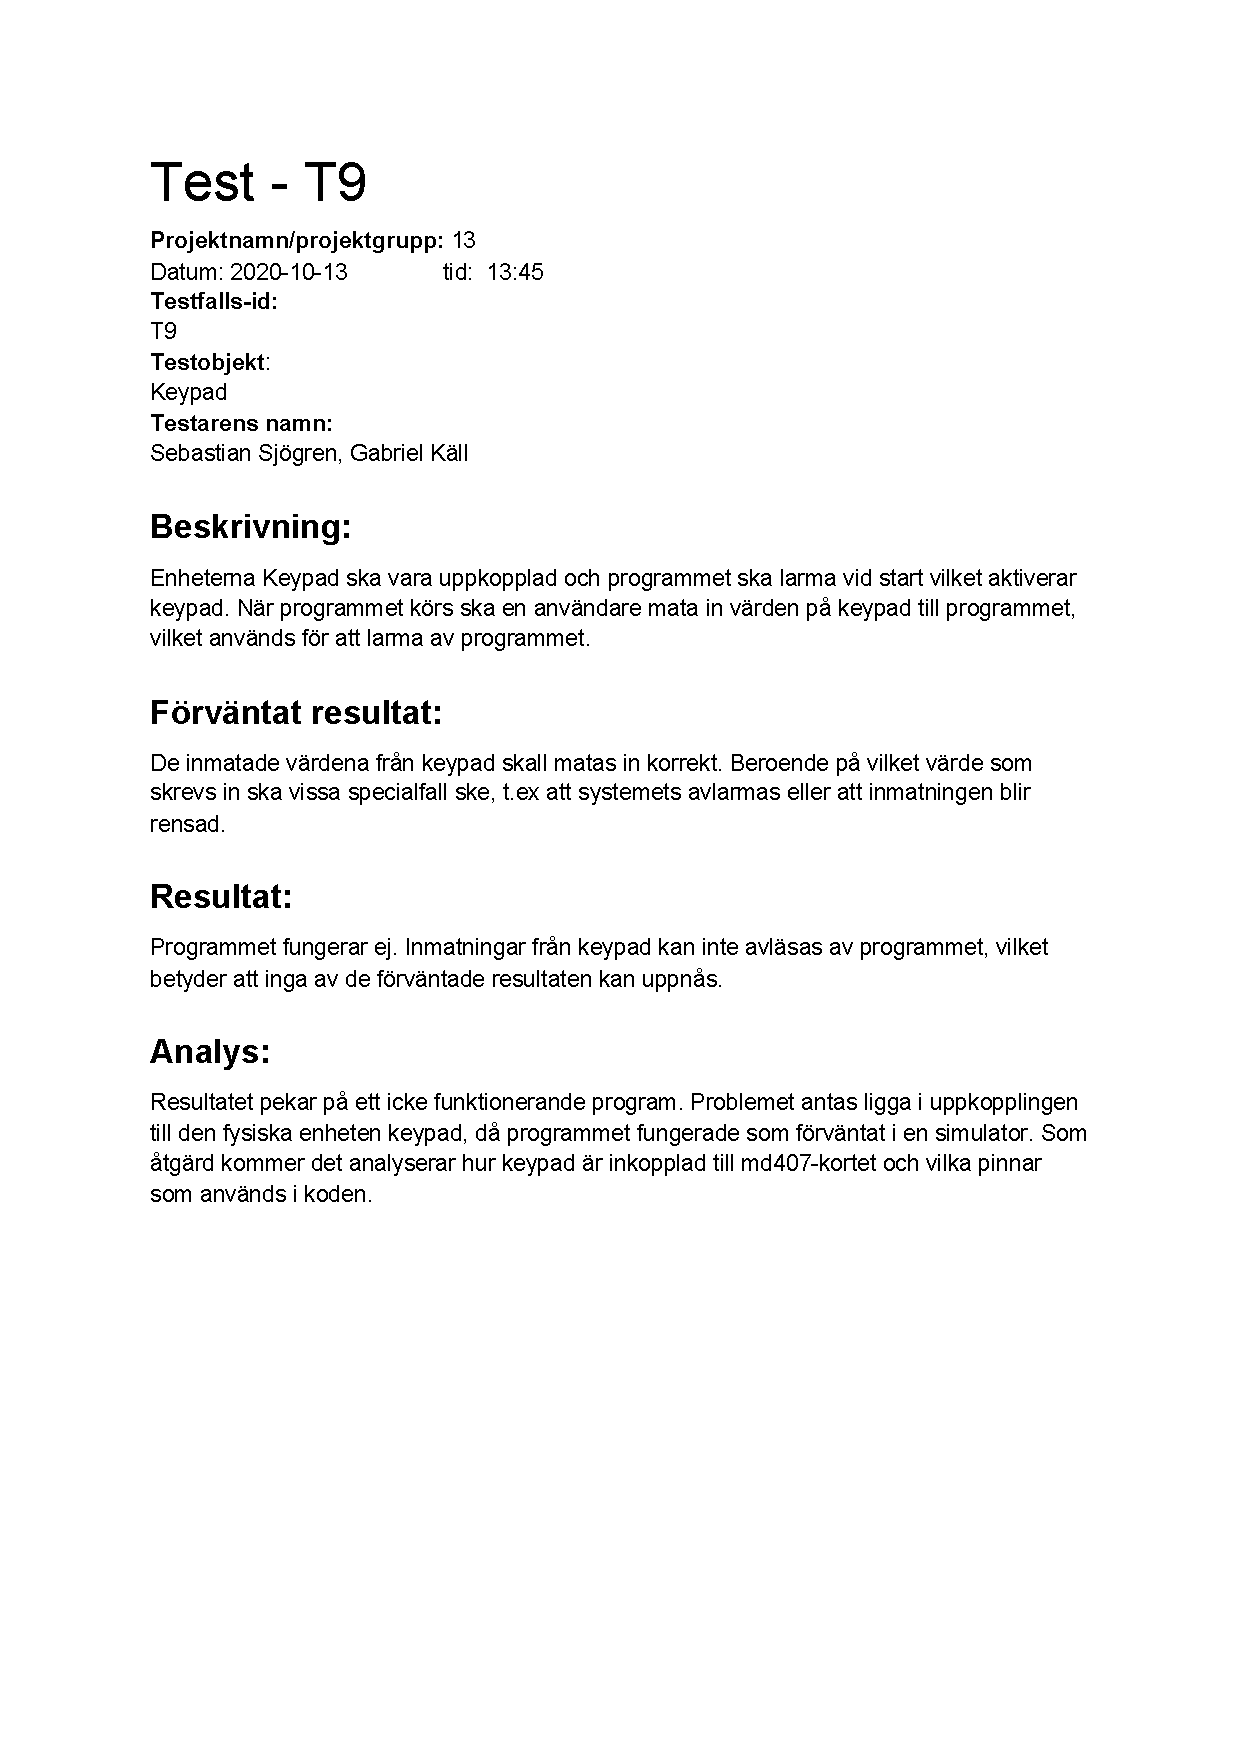
\includepdf{dokumentation/projektrapport/TESTS/Keypad_Test-T9.pdf}
\label{bil:T9}

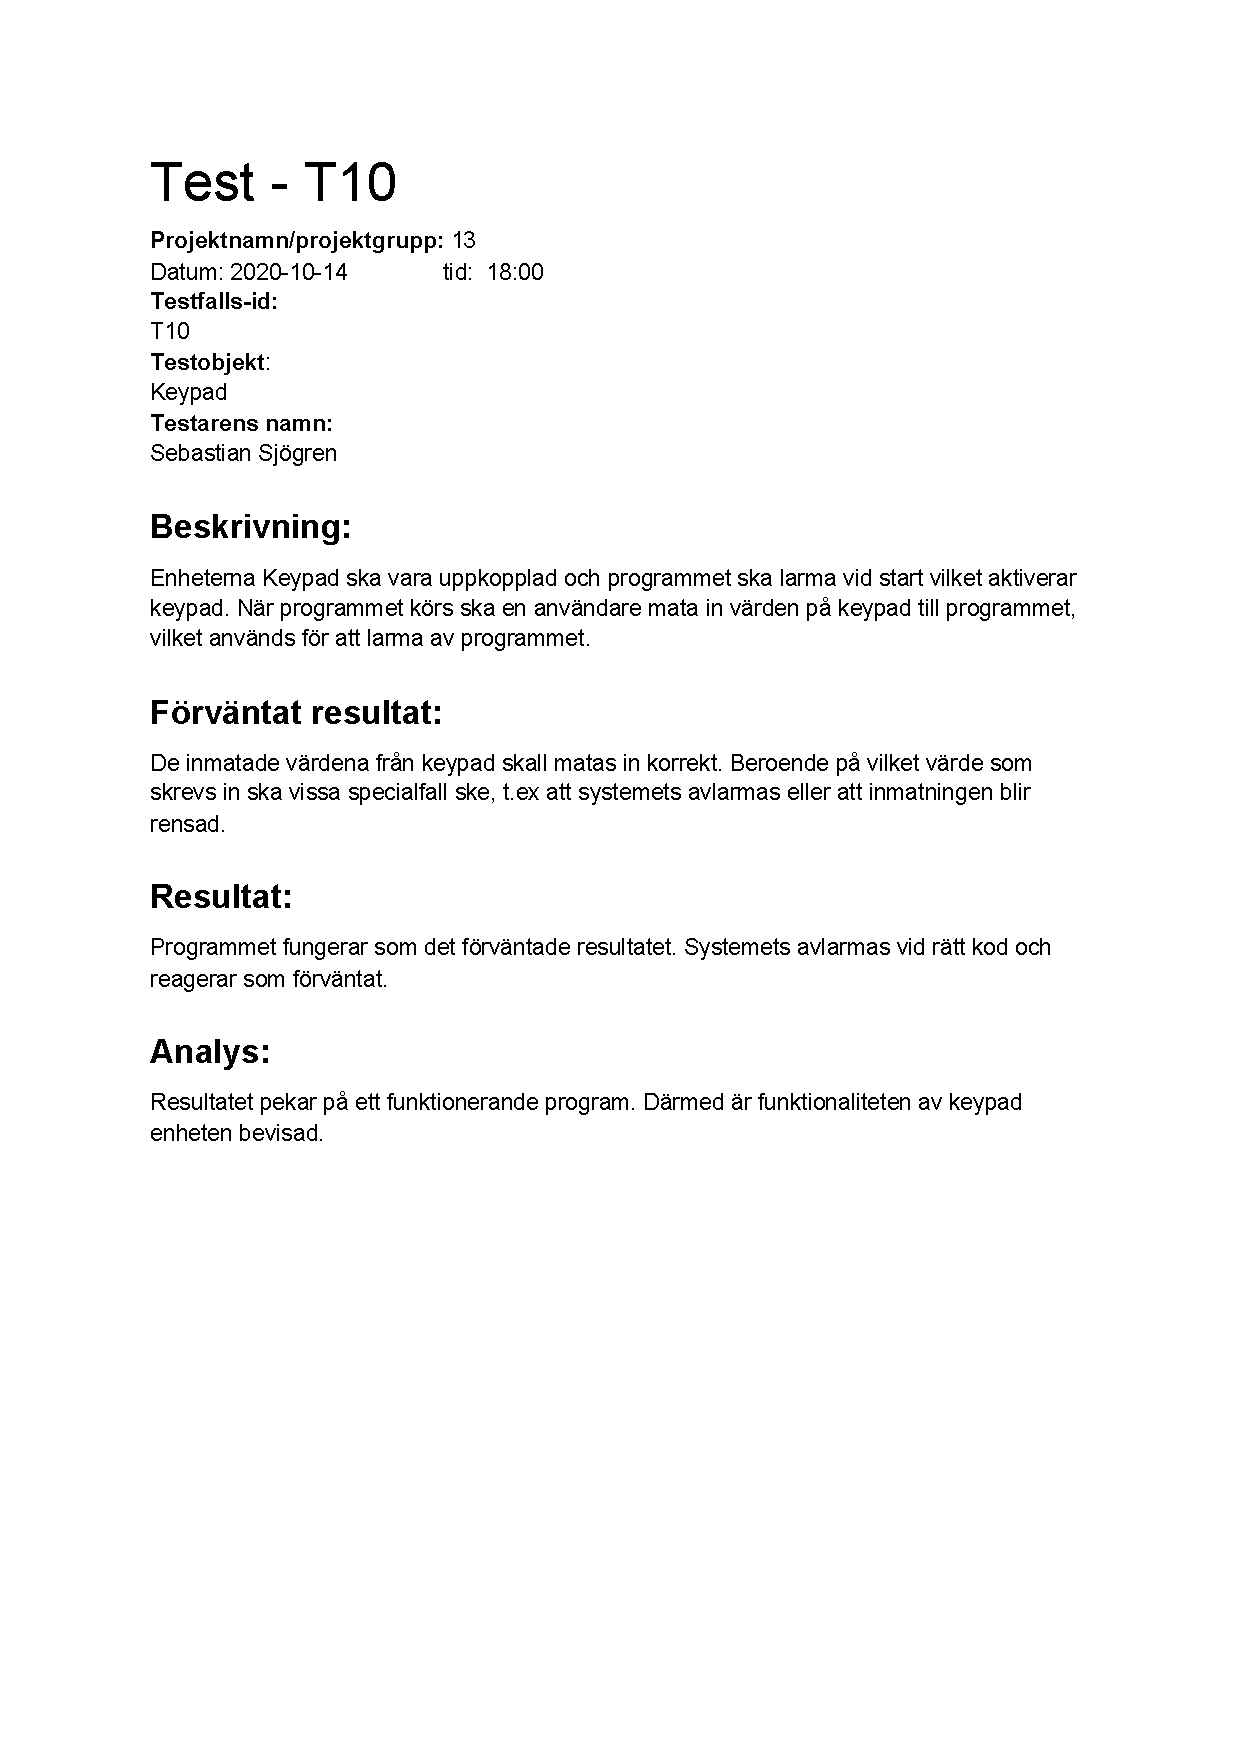
\includepdf{dokumentation/projektrapport/TESTS/Keypad_Test-T10.pdf}
\label{bil:T10}

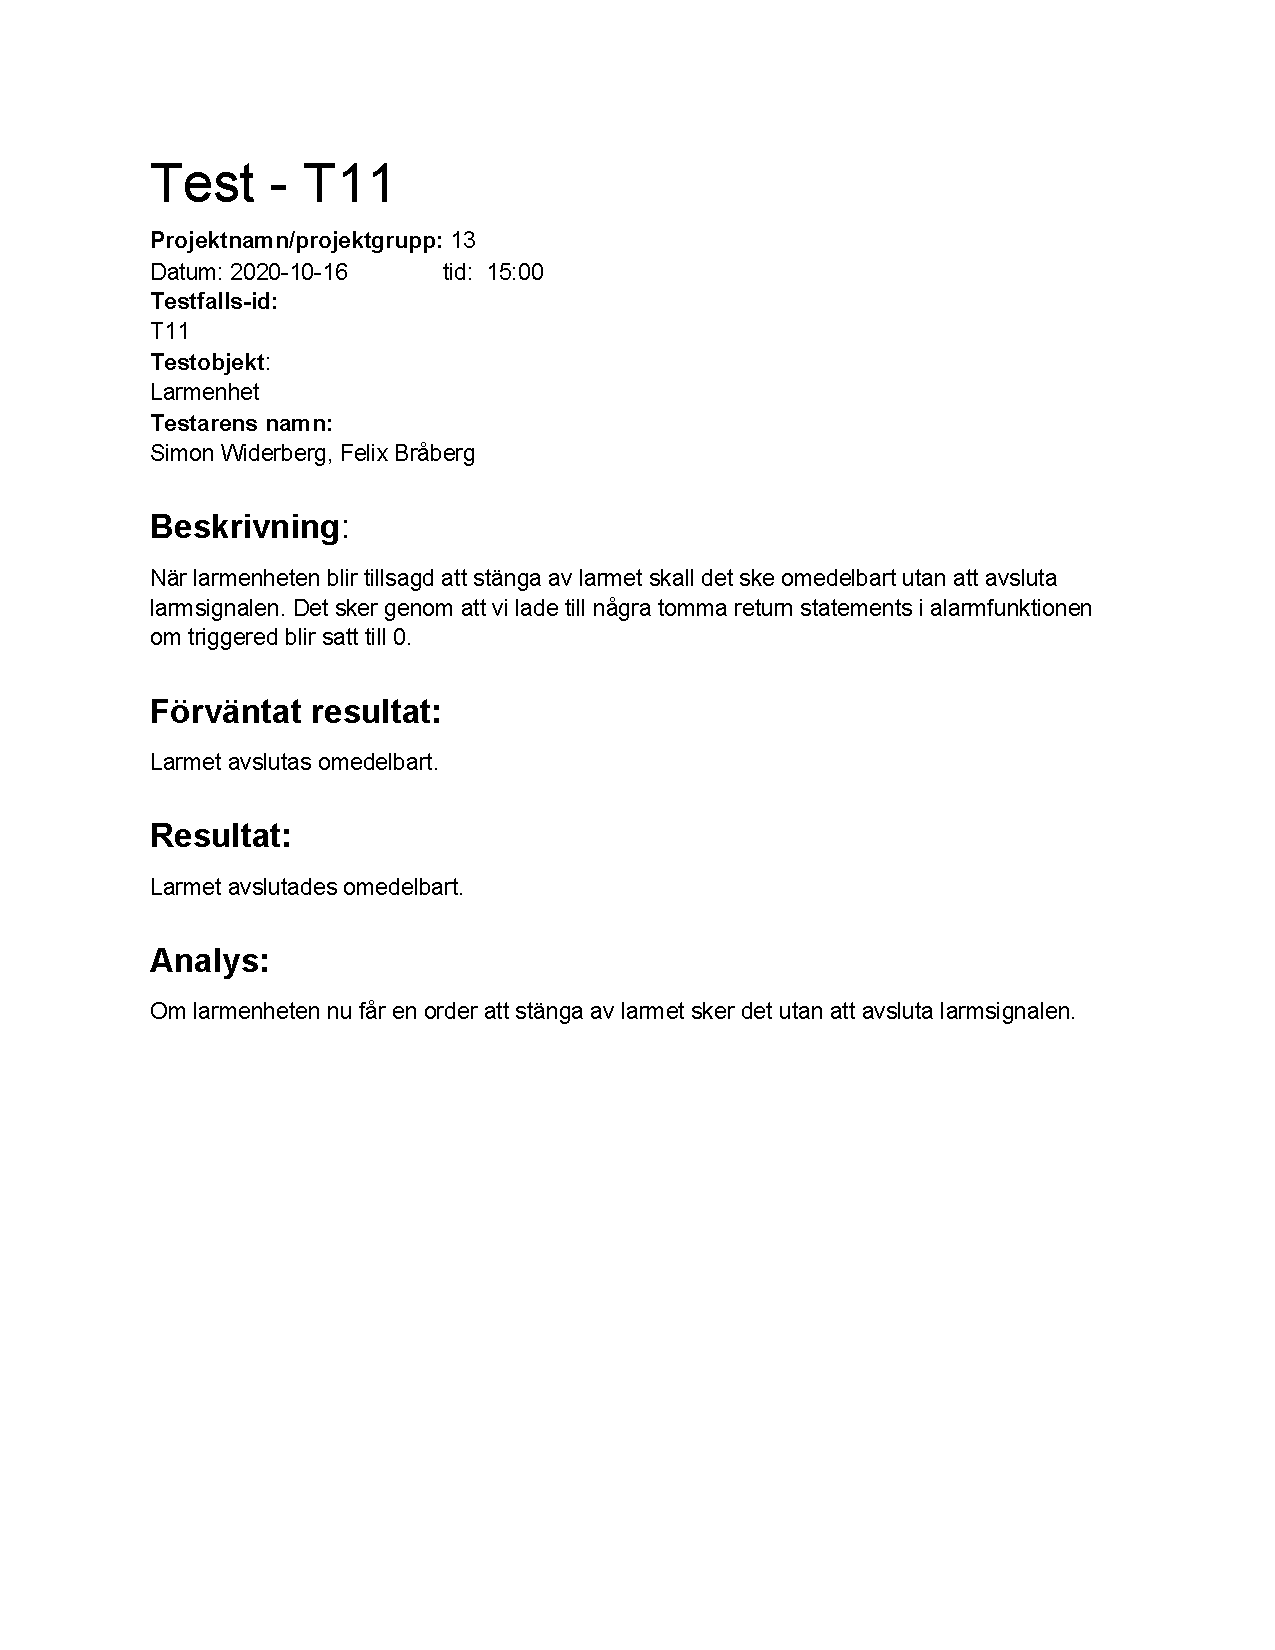
\includepdf{dokumentation/projektrapport/TESTS/Larmenhet_Test-T11.pdf}
\label{bil:T11}

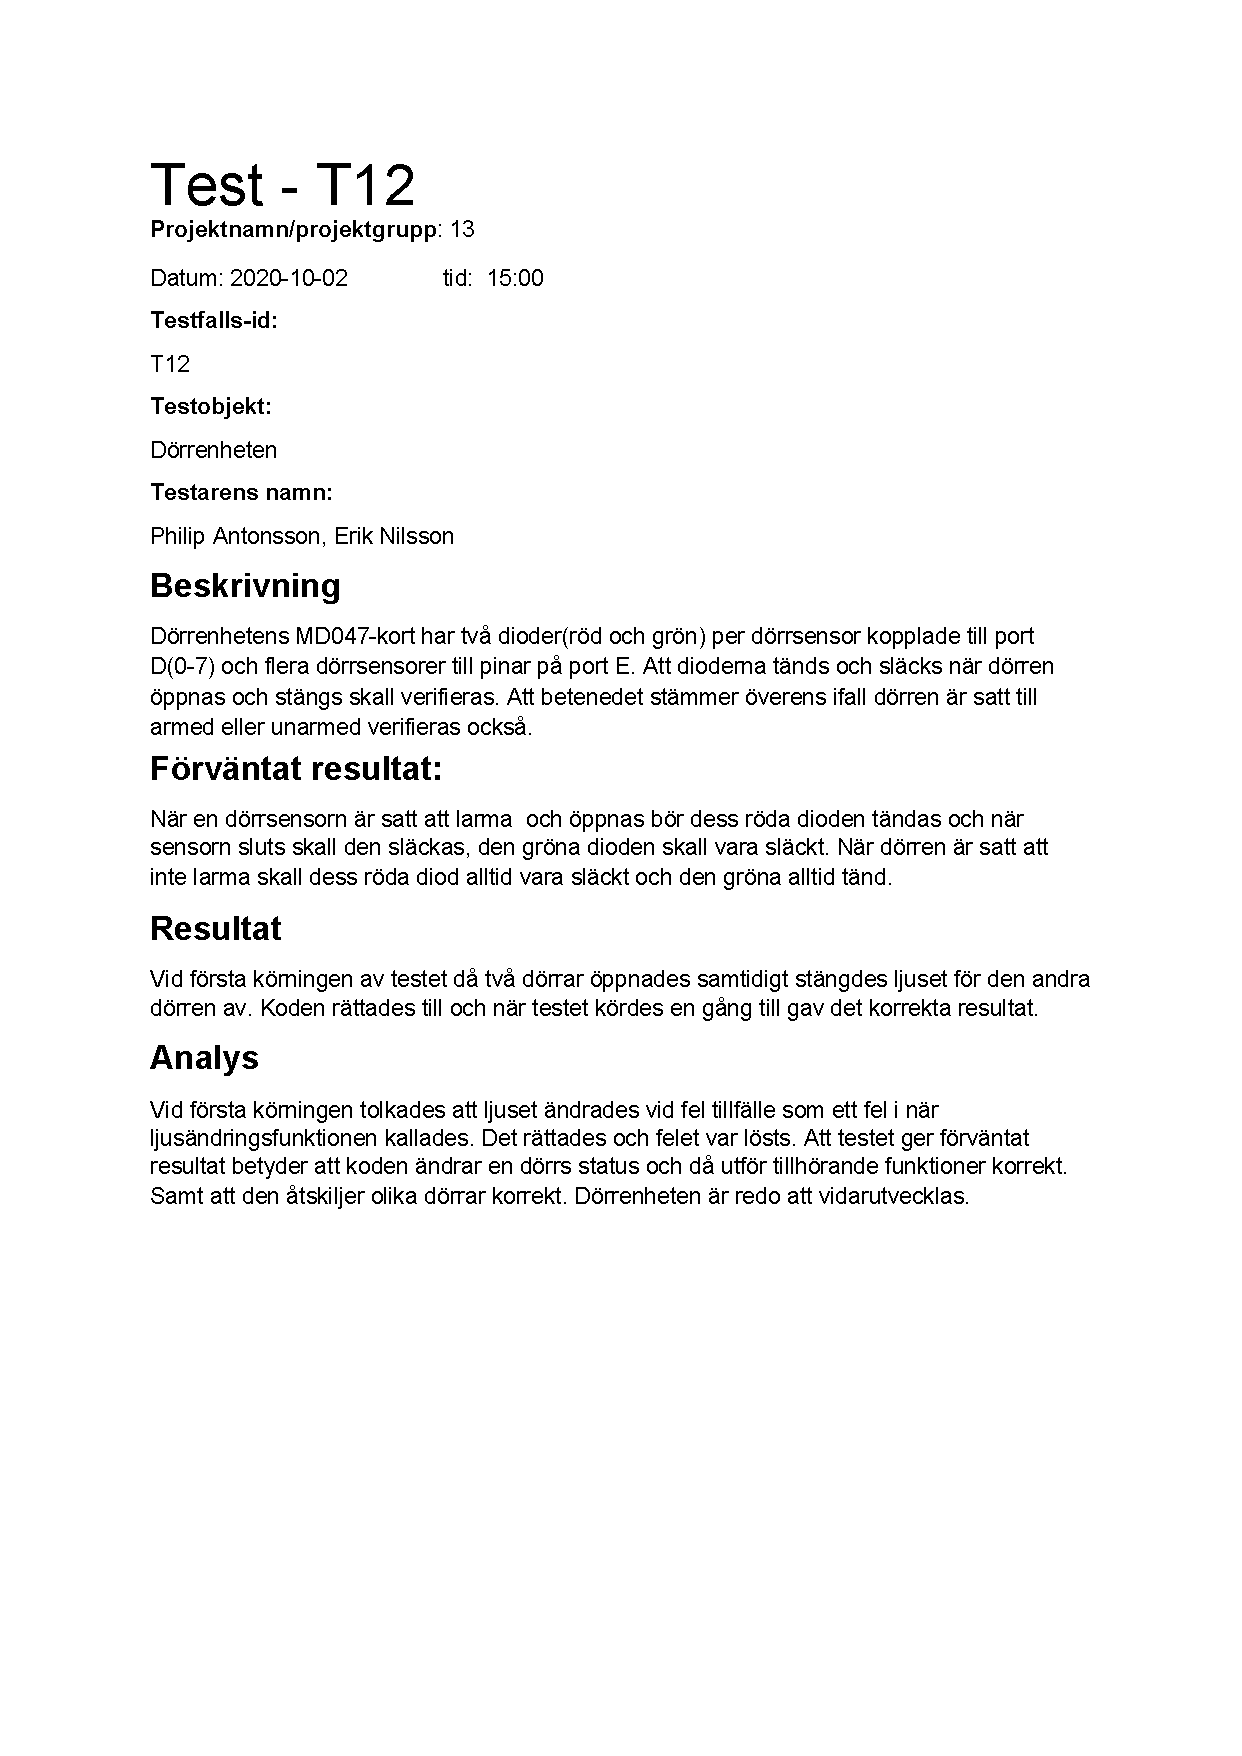
\includepdf{dokumentation/projektrapport/TESTS/Dorrenhet_Test-T12.pdf}
\label{bil:T12}

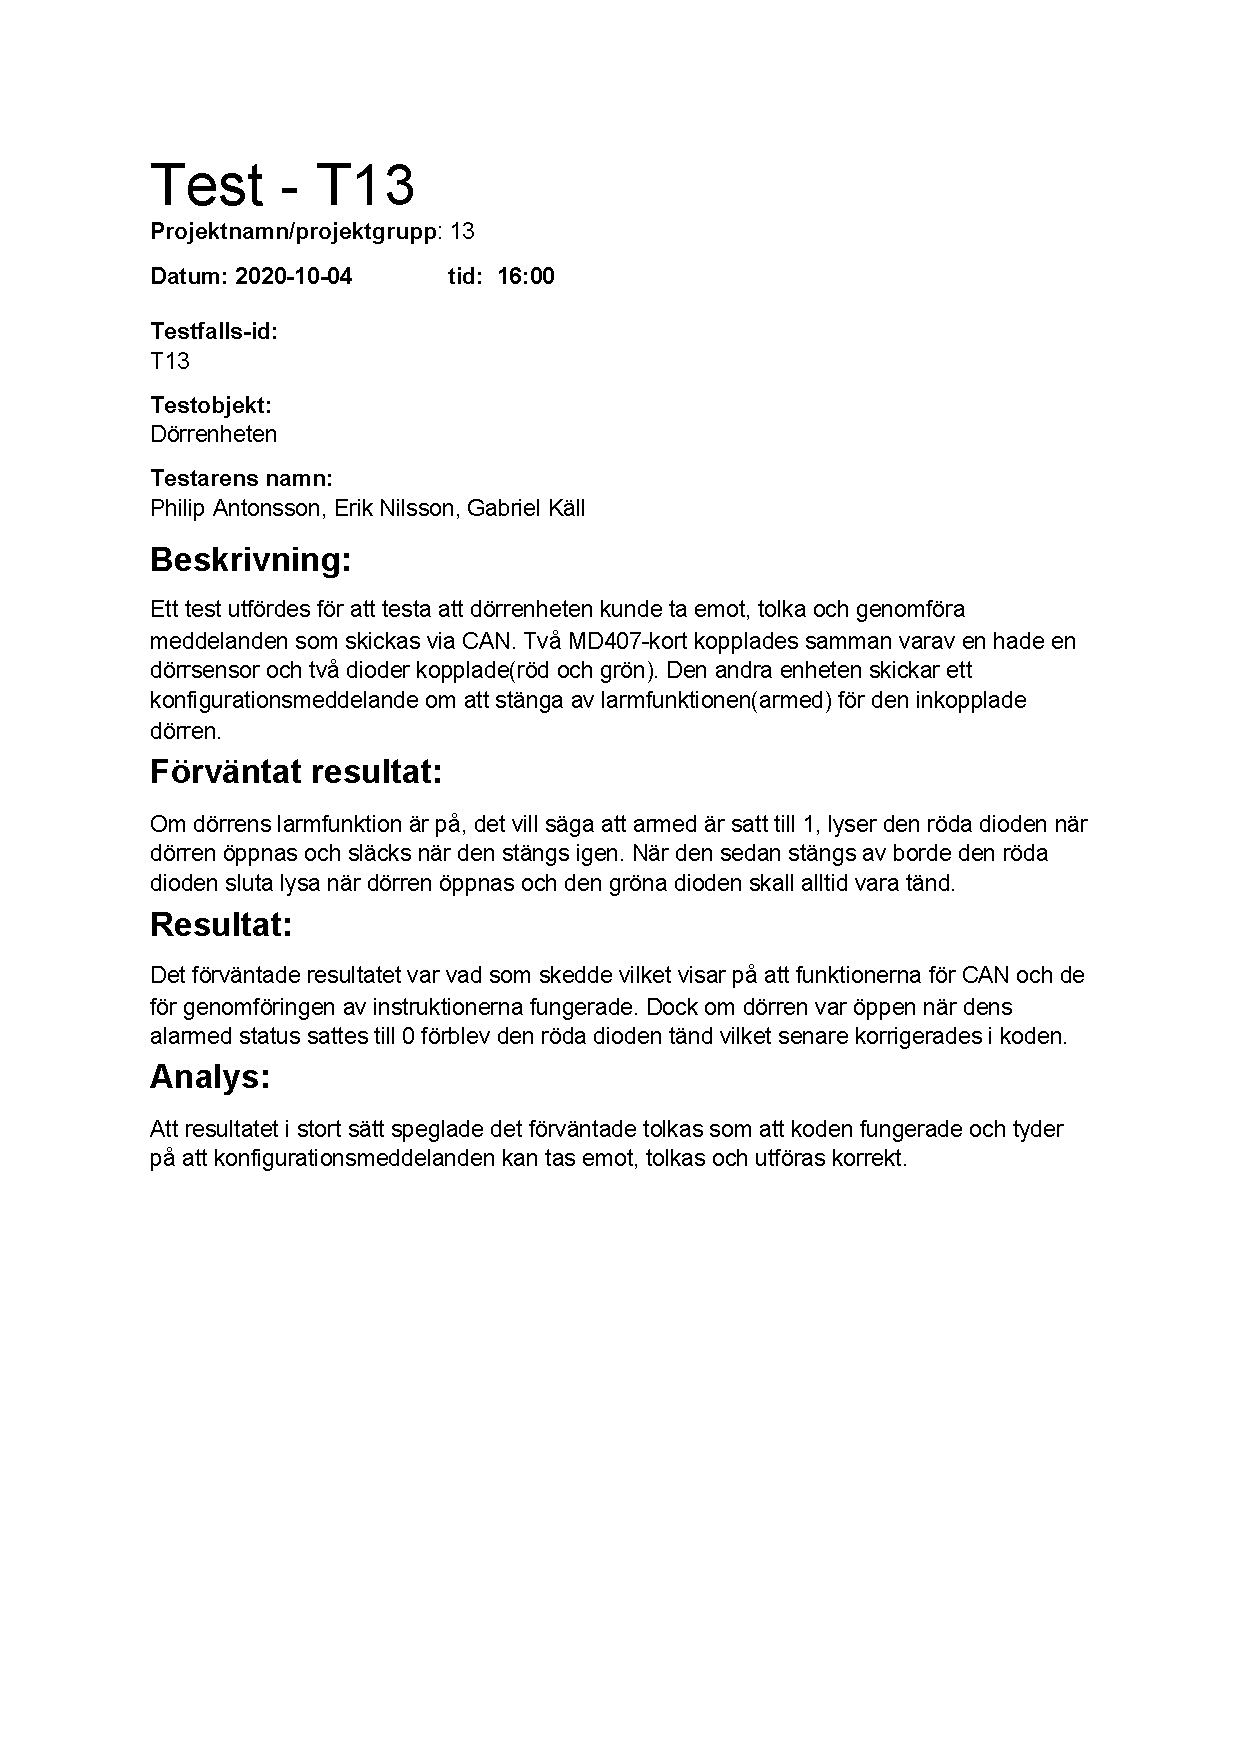
\includepdf{dokumentation/projektrapport/TESTS/Dorrenhet_Test-T13.pdf}
\label{bil:T13}

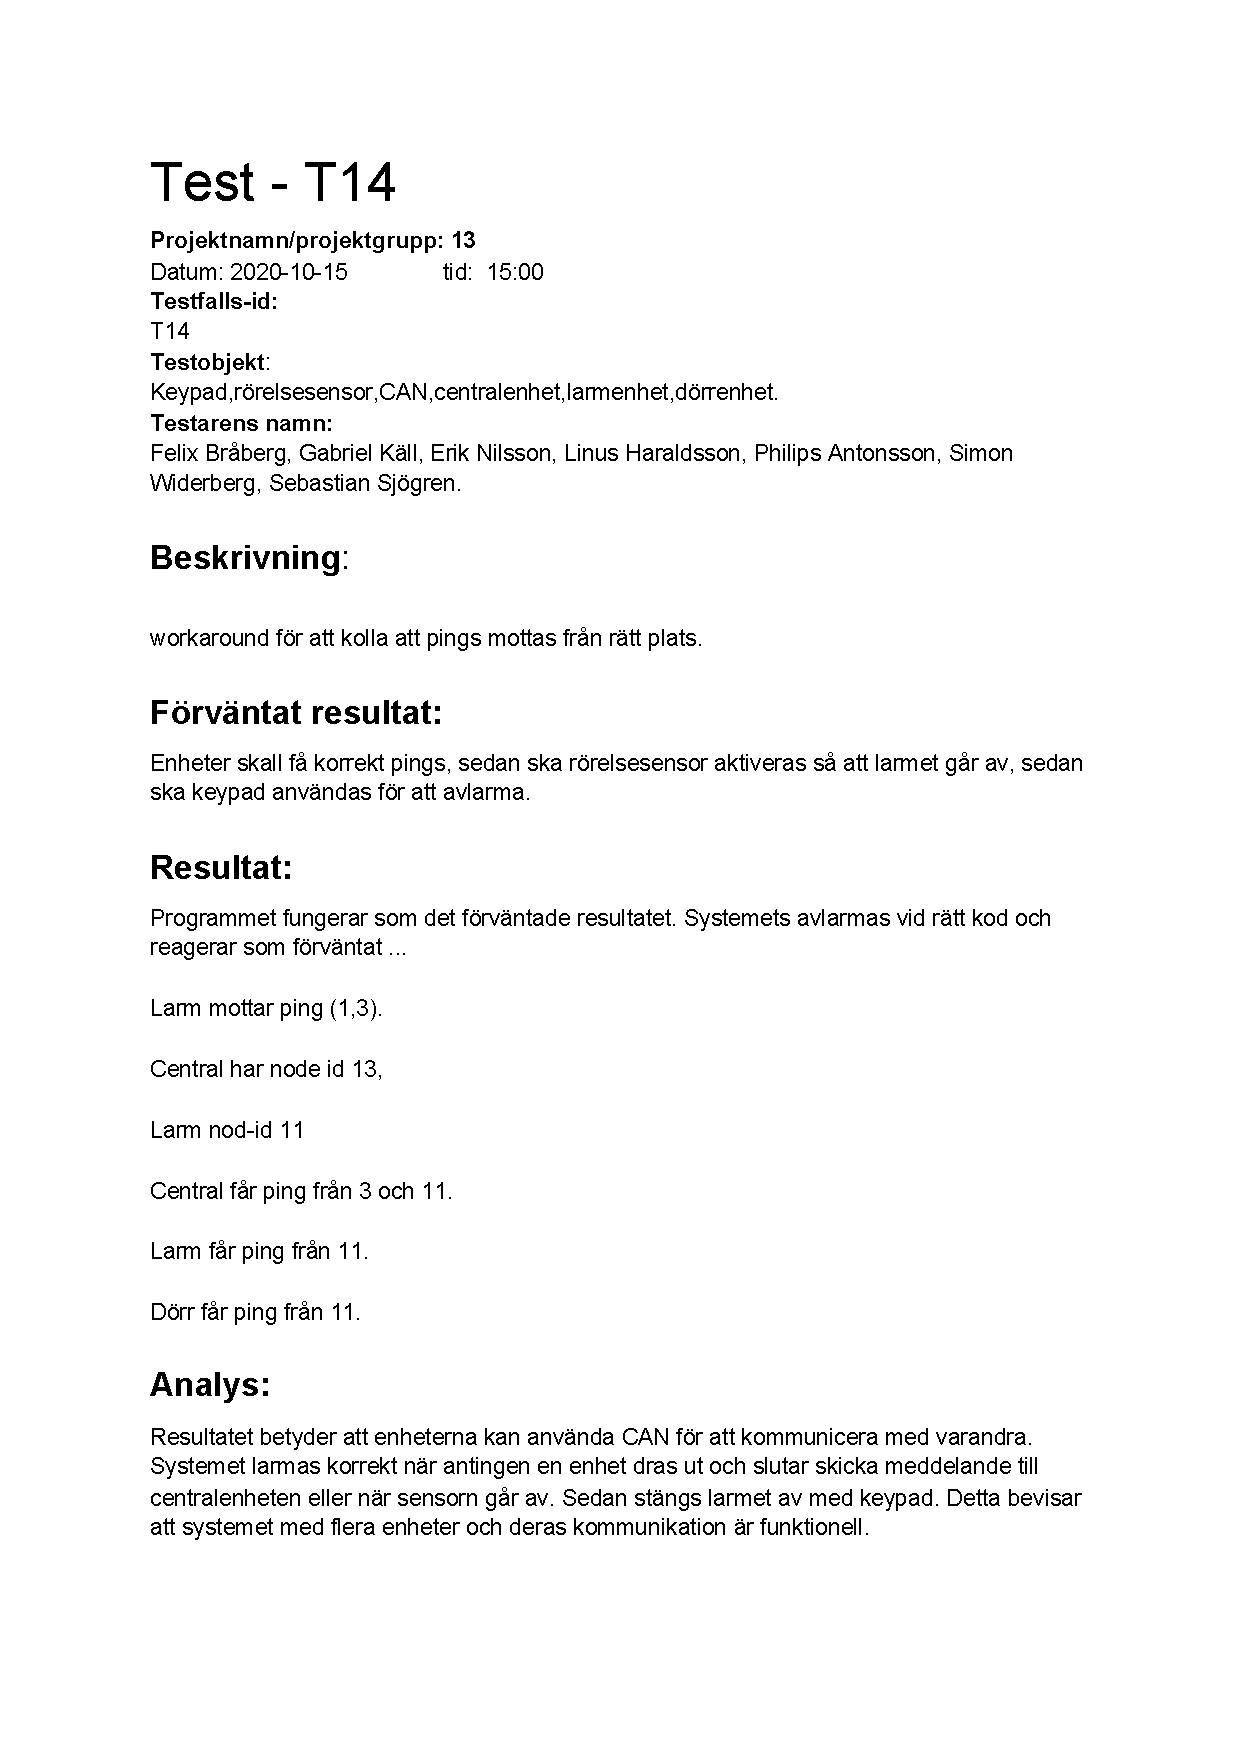
\includepdf{dokumentation/projektrapport/TESTS/System_Test-T14.pdf}
\label{bil:T14}

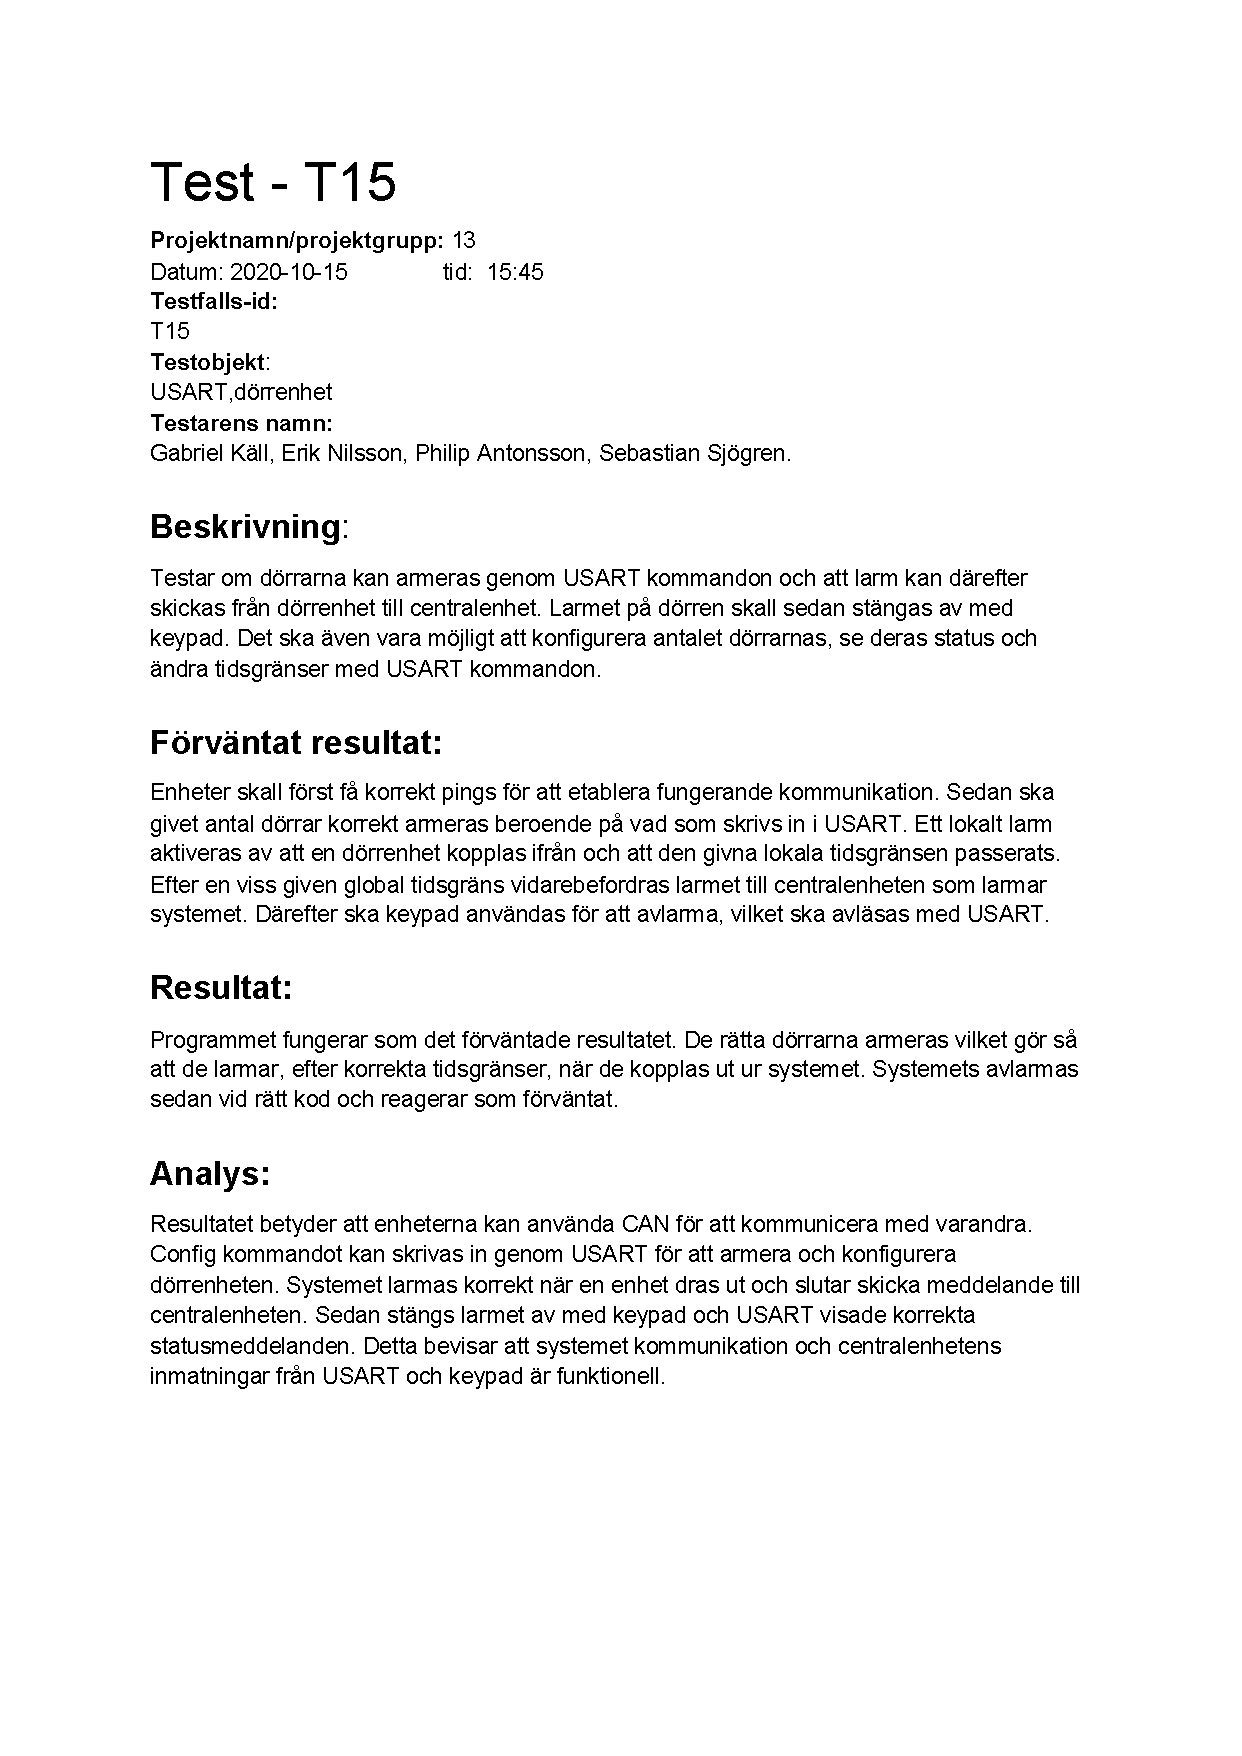
\includepdf{dokumentation/projektrapport/TESTS/USART_DorrenhetTest-T15.pdf}
\label{bil:T15}

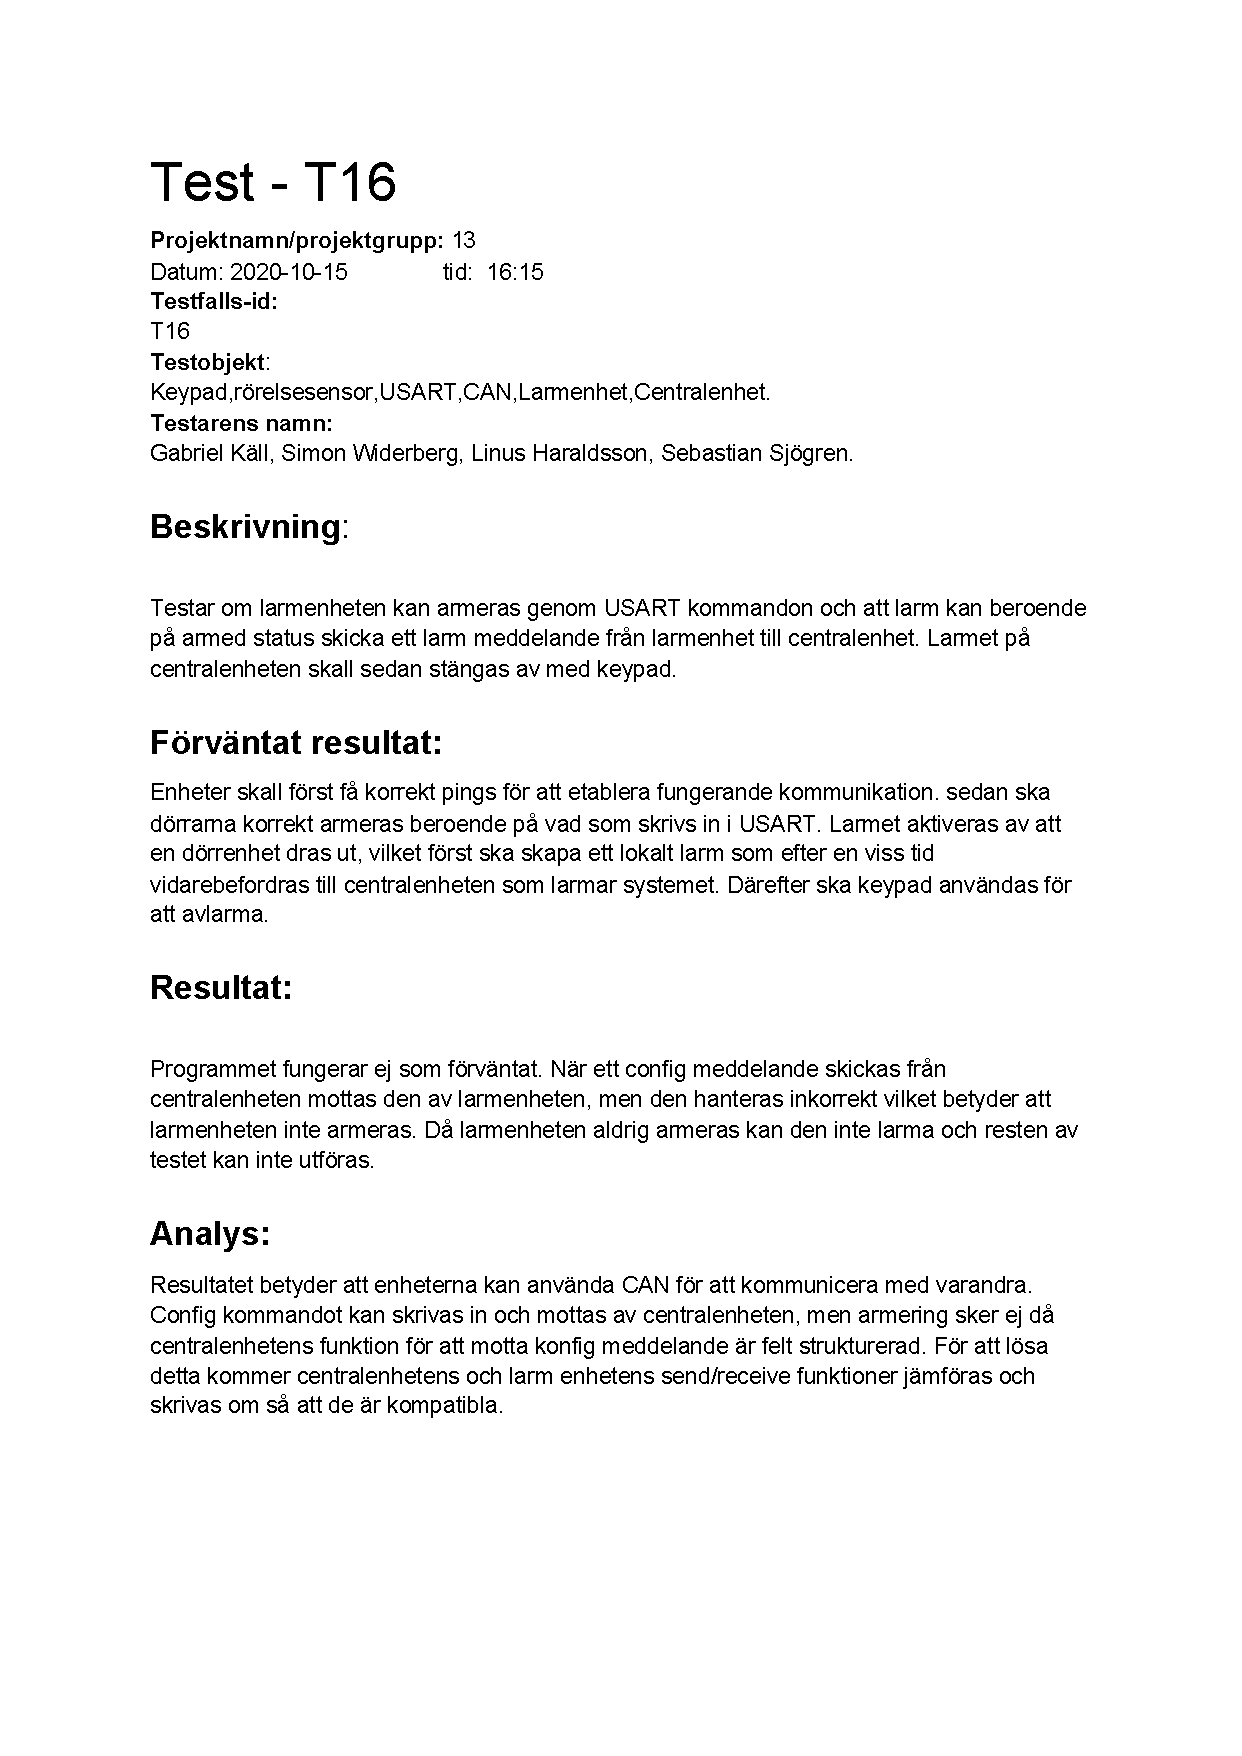
\includepdf{dokumentation/projektrapport/TESTS/Larmenhet_Test-T16.pdf}
\label{bil:T16}

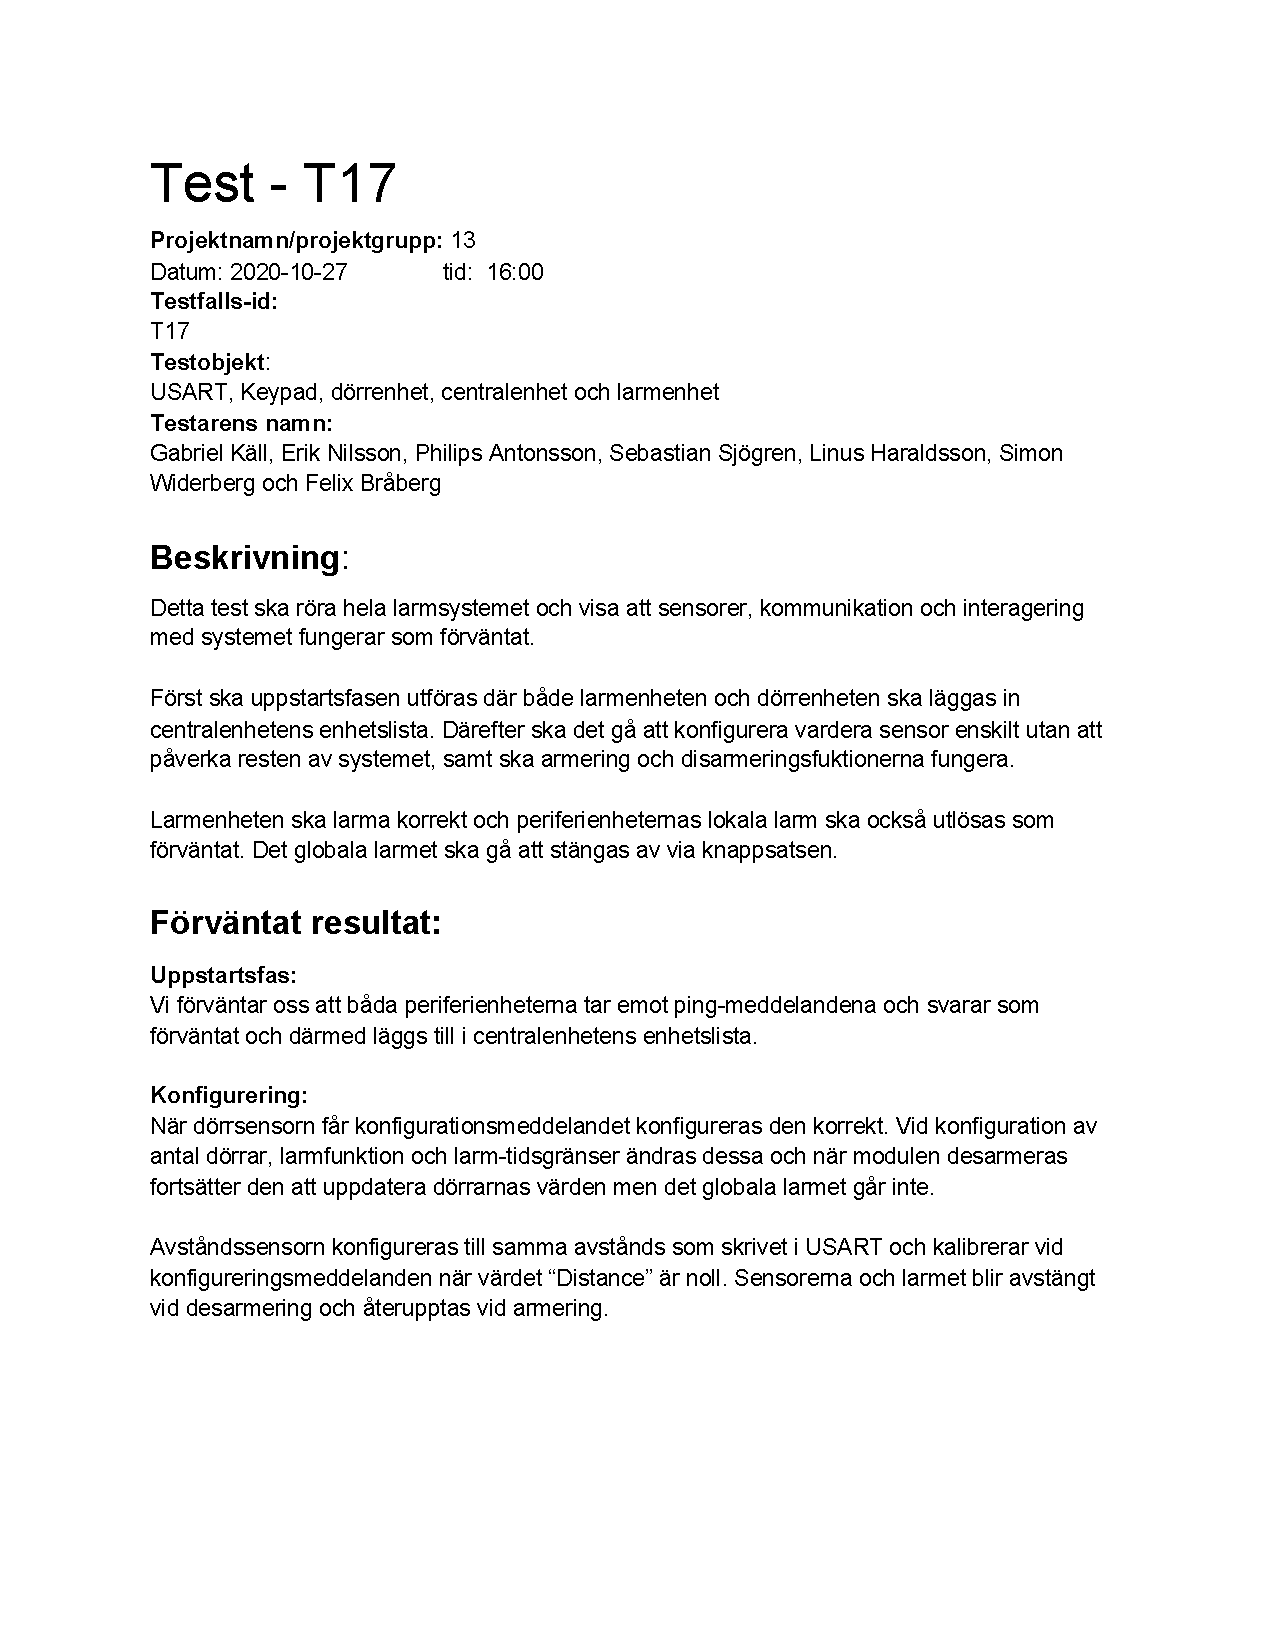
\includepdf[pages={1,2}]{dokumentation/projektrapport/TESTS/Helhetstest-T17.pdf}
\label{bil:T17}


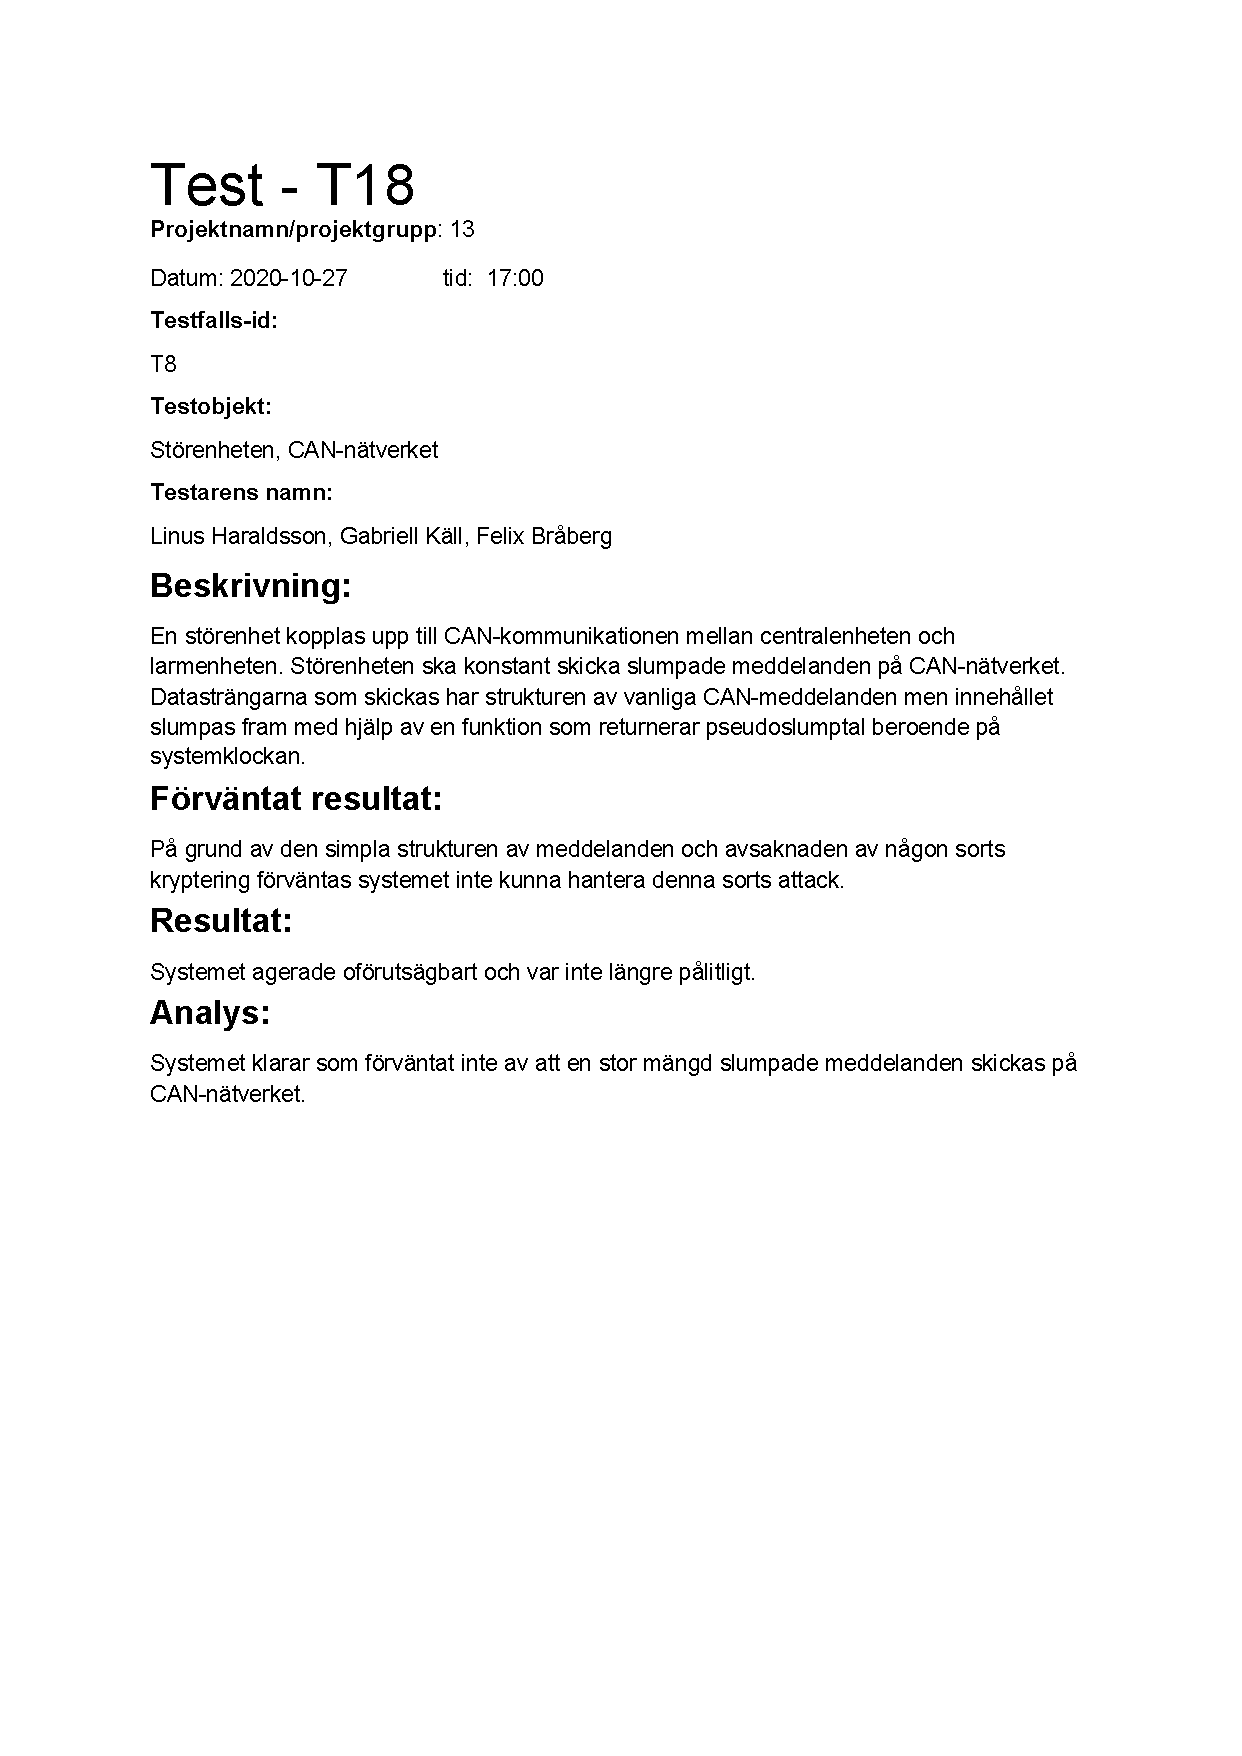
\includepdf{dokumentation/projektrapport/TESTS/Storenhet_Test-T18.pdf}
\label{bil:T18}

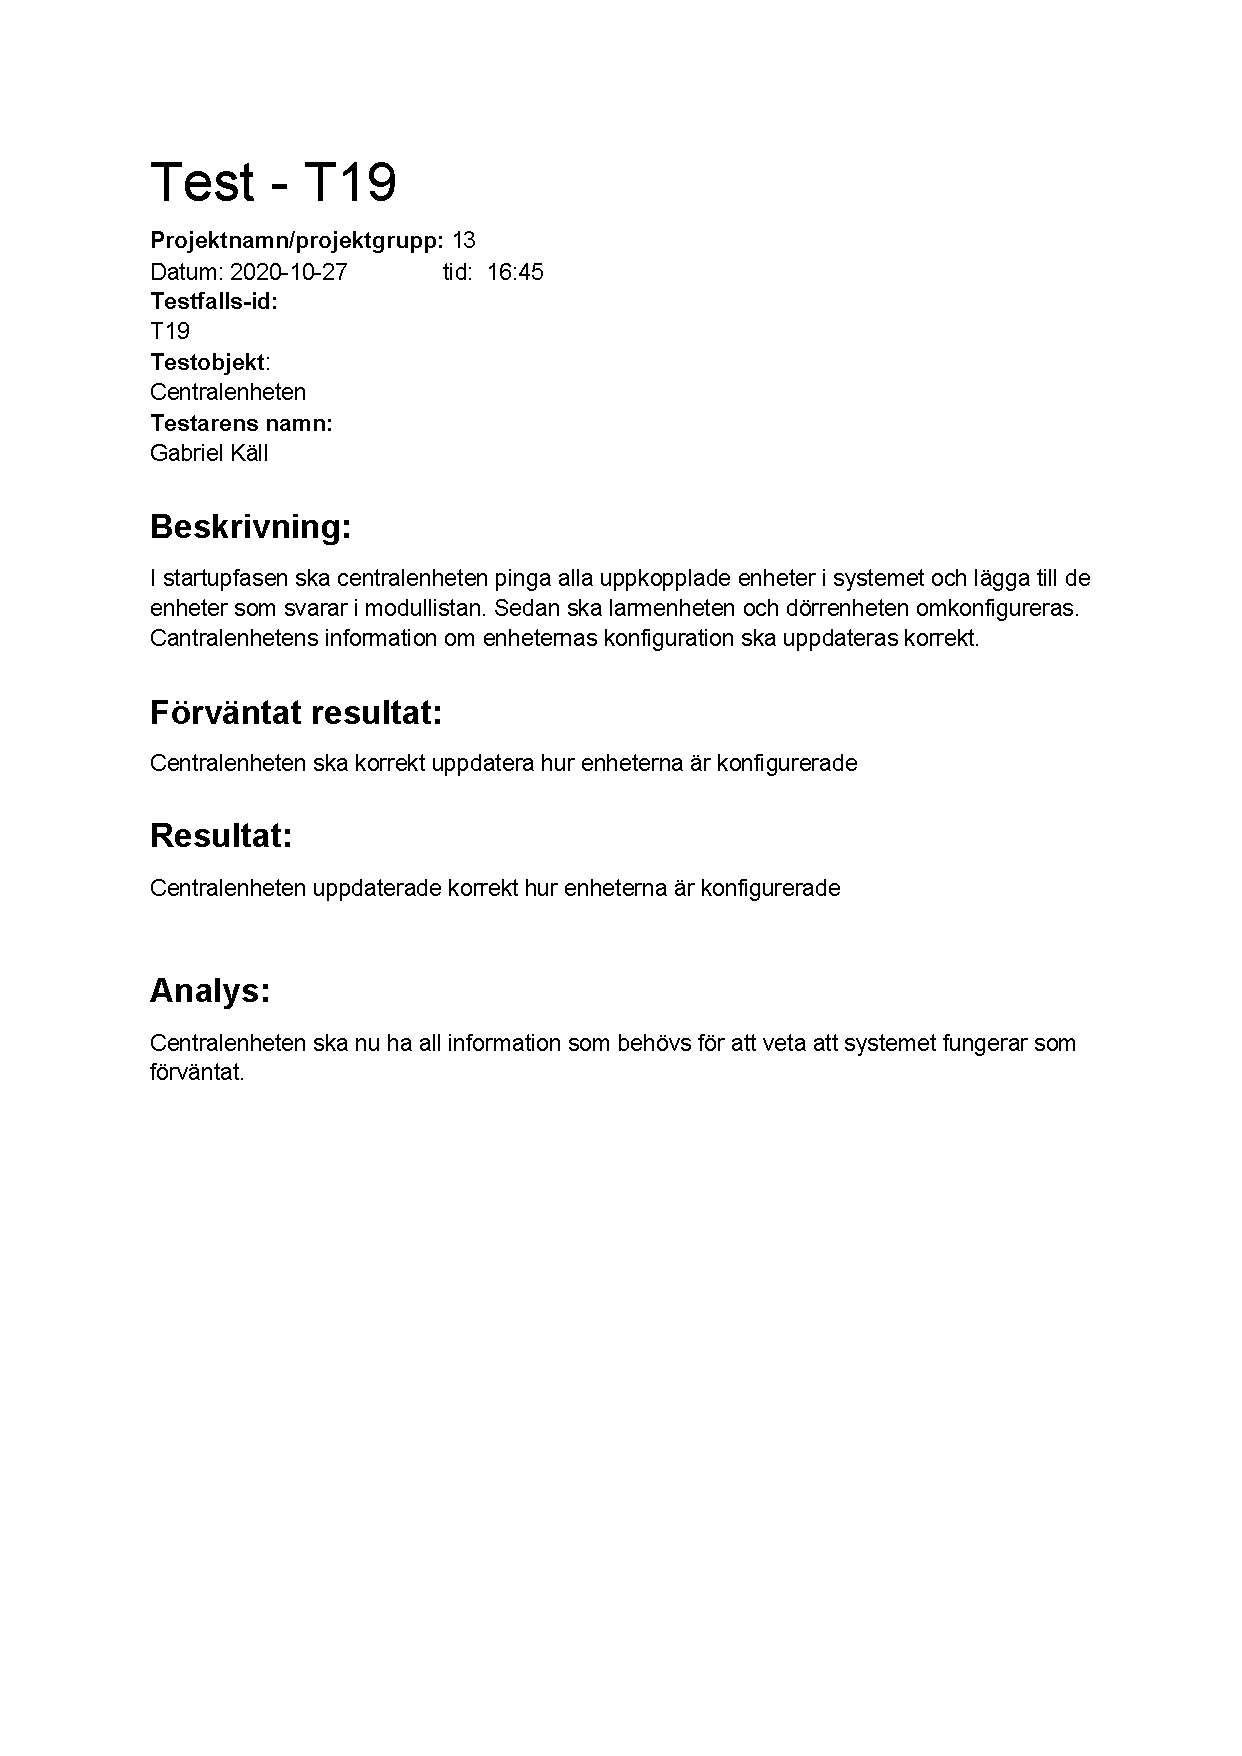
\includepdf{dokumentation/projektrapport/TESTS/Centralenheten_Test-T19.pdf}
\label{bil:T19}
\end{document}
